\documentclass{article}
\usepackage{graphicx} % Required for inserting images
\usepackage{amsmath,amssymb}
\usepackage{enumerate}
\usepackage{dcolumn}
\usepackage{bm}
\usepackage{microtype}
\usepackage{xcolor}
\usepackage{bbold}
\usepackage{soul}



\definecolor{navyblue}{rgb}{0.0, 0.0, 0.5}
\usepackage{hyperref}
\usepackage{cleveref} 
\hypersetup{
    colorlinks=true,
    linktoc=all,
    allcolors=navyblue
}

\bibliographystyle{ieeetr}

\title{Axiverse Machine}
\author{Masha Baryakhtar, David Cyncynates, Ella Henry}
\date{\today}

\begin{document}

\maketitle

\section{Anthropics}
The bounds for the possible ratio of the dark matter abundance to baryon abundance, $\zeta$, are given in \cite{anthropic-explanation} to be $2.5<\zeta <100$. The lower bound is related to the value for which perturbations near the size of our galaxy's stop growing, and the upper bound is related to the value that ultimately prevents star formation. All values within this range are allowed in the sense that they would lead to our existence today, but their likelihoods depend on the theory for dark matter, as we will see below. In section 5 of \cite{exploring-string-axiverse}, the authors consider the case of $n$ axions and the fraction of the dark matter that they constitute. If the axions make up all of the dark matter, then we can write $\zeta$ as:

\begin{equation}
\label{eq:zeta}
    \zeta = \sum_{a=1}^n c(m_a) F(\theta_a)
\end{equation}

Here, $c(m_a)F(\theta_a)$ is the fractional abundance in the $a$-th axion, where $F(\theta_a)$ encodes the dependence of the fractional abundance on the axion's intial misalignment angle. For small enough angles, $F(\theta_a)\sim\theta_a^2$. The $c(m_a)$ factor takes into account the fractional abundance's dependence on the mass and on the scale of symmetry breaking, e.g. for axions that start to oscillate during radiation domination, $c(m_a) \sim \Big(\frac{m_a}{H_{eq}}\Big)^{1/2}\Big(\frac{f_a}{M_{pl}}\Big)^2$.

\subsection{The anthropic measure}

The authors of \cite{exploring-string-axiverse} then calculate the probability $P$ of finding ourselves in a causal patch where the dark matter abundance is no larger than the observed value of $\zeta \sim 5$, without being so small that we could not exist, in other words, the probability that $2.5<\zeta<5$. The calculation uses the causal diamond measure (details in \cite{anthropic-explanation}) to circumvent the problem of computing probabilities in an infinite-dimensional space, which leads to difficulties in normalizing these probabilities. The measure allows us to restrict ourselves to one causal patch and consider the number of observations made in that patch. To determine this number, the author of \cite{anthropic-explanation} counts the number of baryons in a causal patch and then the number of observations per baryon. The quantitative expression the author finds for the number of baryons in a causal patch is $(1+\zeta)^{-1}$ with the assumption of fixed baryon-to-photon ratio. The number of observers per baryon is approximated to be constant within the range of allowed $\zeta$ values. The overall contribution to the probability density from the causal diamond measure is therefore $C(1+\zeta)^{-1}$, for some constant $C$.

We must also assume some distribution for the initial conditions $\theta_a$, which will depend on the scale of inflation relative to the axion's potential: for high scale inflation, the distribution is flat between $[-\pi,\pi]$, while for low scale inflation,     $p(\theta_a) \propto \exp{\left(-\frac{8\pi^2V(\theta_a)}{3H^4}\right)}$, where $V(\theta_a)=\Lambda^4(1-\cos{\theta_a})$. We can approximate this distribution from low scale inflation as flat between $[-\sigma,\sigma]$, where $\sigma^2 = 3H^4/(8\pi^2m^2f^2)$ is the spread in this distribution. So in general, we can consider $p(\theta_a)$ to be flat between two values, which we'll call $\pm f(H)$, where:

\begin{equation}
\label{eq:f(H)}
    f(H) = \begin{cases}
        \pi \; \text{ for } H>\Lambda\\
        \sigma \; \text{ for } H < \Lambda
    \end{cases}
\end{equation}

Now, using the causal diamond measure described above and the flat distribution between $\pm f(H)$ for the initial conditions, we can write down an expression for the probability $P$:

\begin{equation}
    \label{eq:prob-deriv}
    P = N^{-1} \frac{C}{(2f(H))^n}\int_{2.5<\zeta(\theta_a)<5} \frac{\prod_{a=1}^nd\theta_a}{1+\zeta(\theta_a)}
\end{equation}

\noindent where again $n$ is the number of axions and $C$ is the constant factor from the number of observations per baryon. The normalization $N$ is such that the probability is normalized to 1 and is given by:

\begin{equation}
    \label{eq:prob-deriv-norm}
    N = \frac{C}{(2f(H))^n}\int_{2.5<\zeta(\theta_a)<100} \frac{\prod_{a=1}^nd\theta_a}{1+\zeta(\theta_a)}
\end{equation}

We can compute this probability for any value of $f(H)$ by rescaling the integration variables as $\theta_a' = \theta_a/f(H)$ and writing $\zeta(\theta_a)=c_a\theta_a^2$ (summing over the $a$ index):

\begin{equation}
    \label{eq:general-prob}
     P = \mathcal{N}^{-1} \int_{-1}^1 \frac{\prod_{a=1}^nd\theta_a'}{1+c_a'\theta_a'^2}\Theta(c_a'\theta_a'^2-2.5)\Theta(5-c_a'\theta_a'^2)
\end{equation}

\noindent where the $\theta_a$-independent factors out front in Eq. \eqref{eq:prob-deriv} have canceled out with those in the normalization $N$, and so $\mathcal{N}$ is the same as $N$, without those factors. $\Theta$ here is the Heaviside function and $c_a'\equiv c_af(H)^2$.

\subsection{1 axion}
\label{subsec:1-axion}

The probability for one axion is given by Eq. $\eqref{eq:general-prob}$ for $n=1$ and can be computed numerically as a function of $c_1$. It is plotted below:

\begin{figure}[h]
    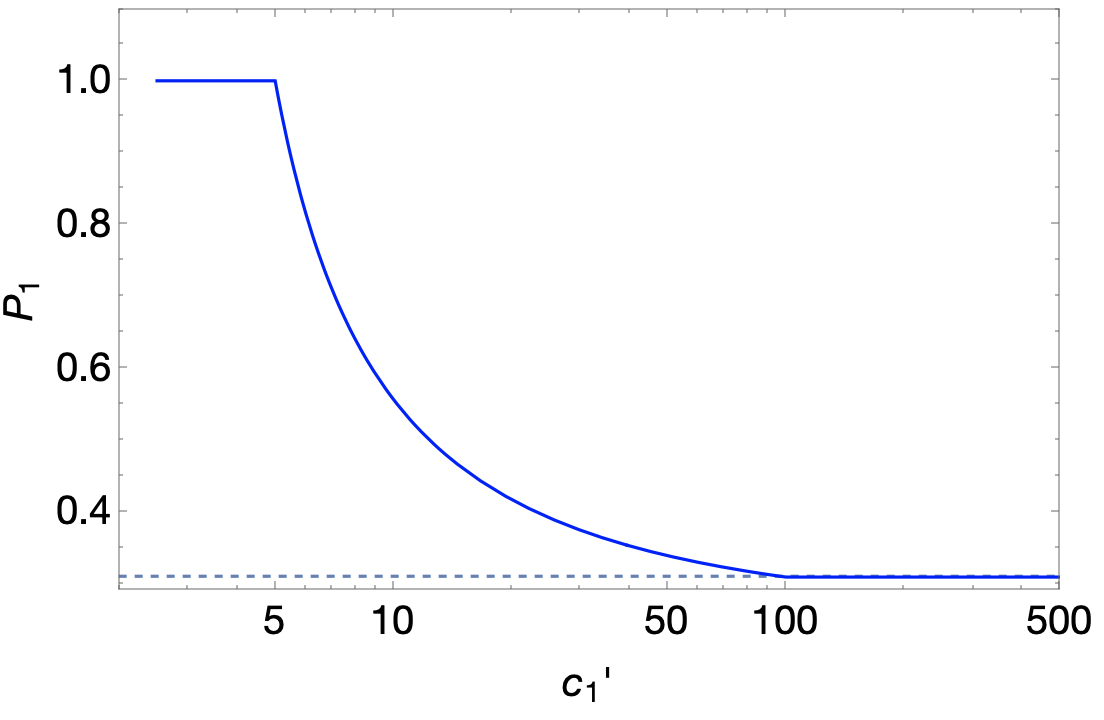
\includegraphics[scale=0.5]{figs/1axion-prob.jpeg}
    \centering
    \caption{Probability of measuring $2.5<\zeta<5$ in the case of one axion, as a function of $c_1'$. The dashed horizontal line corresponds to $P=0.3$, the probability found for 1 axion in \cite{exploring-string-axiverse}}.
    \label{fig:1axion-prob}
\end{figure}

Fig. \ref{fig:1axion-prob} shows that once $c_1'>\zeta_\text{upper}=100$, the probability becomes independent of the axion parameters (recall that $c' \propto m^{1/2}f^2$), and acquires the constant value of $P=0.3$. This corresponds to the $n=1$ case of the result presented in Eq. 79 of \cite{exploring-string-axiverse}, reproduced below:

\begin{equation}
\label{eq:bookkeeping-result}
    P_n = \frac{\int_{2.5}^5 \frac{d\zeta \zeta^{(n-2)/2}}{1+\zeta}}{\int_{2.5}^{100}\frac{d\zeta \zeta^{(n-2)/2}}{1+\zeta}} = \text{0.3, 0.16, 0.06, 0.02, 0.006, . . .}
\end{equation}

\noindent In this result, the authors focus on $n$ axions at the GUT scale ($f\sim 10^{16}$ GeV), with masses heavy enough ( $m_a\geq10^{-19}$ eV) so that the axions would find themselves in this constant $P$ regime. Indeed, one can check that for $f\sim 10^{16}$ GeV and $m_a\geq10^{-19}$ eV, the criterion $c_a>100$ is satisfied.

\subsubsection{Exact anthropic probability with low scale inflation}

\begin{figure}[h]
    \centering
    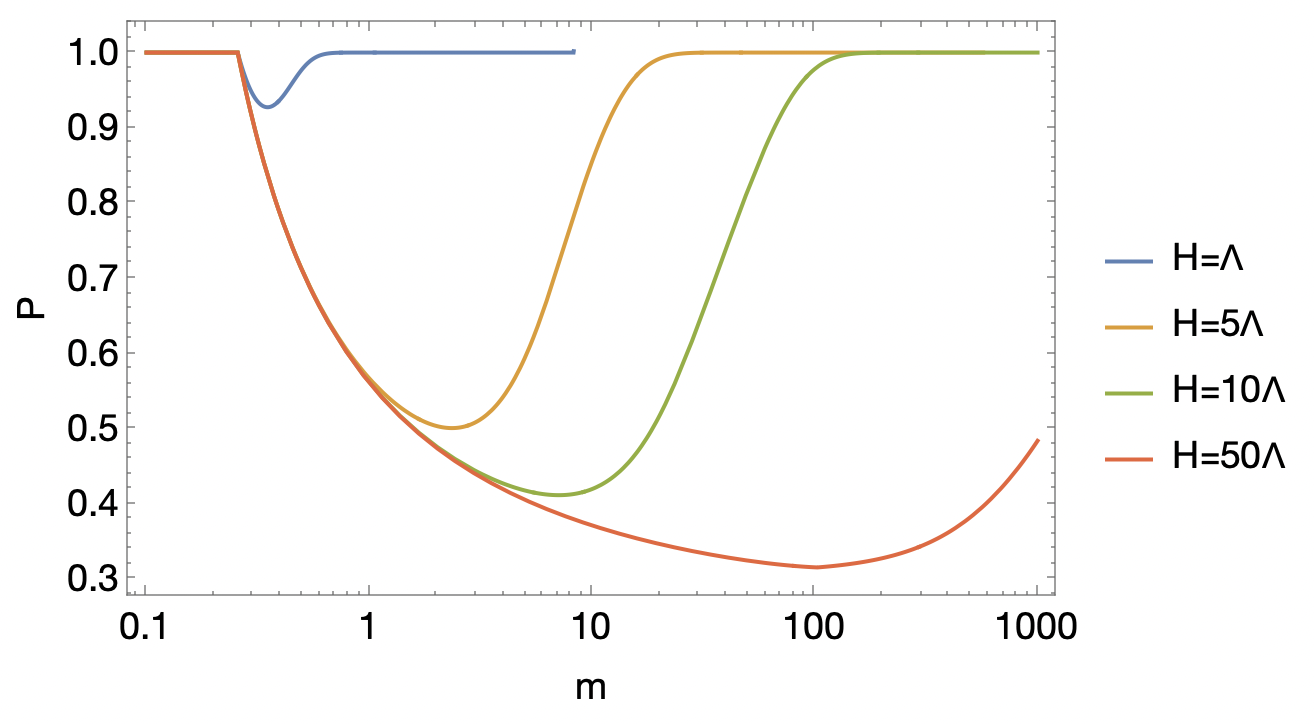
\includegraphics[width=1\linewidth]{figs/low-scale-inf-prob.jpeg}
    \caption{Probability of $2.5<\zeta<5$ for a stochastic axion scenario (low scale, long-lasting inflation), with different vales of $H$ relative to $\Lambda = (mf)^{1/2}$. In this plot, $f=1$.}
    \label{fig:low-scale-inf-prob}
\end{figure}

In Section \ref{subsec:1-axion}, we used an approximate form for the distribution of initial conditions from low scale inflation. We can compute the anthropic probability \textit{for one axion} more precisely in the case of low scale inflation by numerically calculating the following:

\begin{equation}
    \label{eq:inflation-prob-1axion}
    P = N^{-1}\int_{2.5<\zeta<5} \frac{d\theta}{1+\zeta} \exp{\left(-\frac{8\pi^2V(\theta)}{3H^4}\right)}
\end{equation}

\noindent where the normalization is the same integral but with integration bound $2.5<\zeta<100$. This probability is plotted against $\sqrt{mf}$ for certain values of $H$ in Fig. \ref{fig:low-scale-inf-prob} (and $f$ is set to 1).

As expected, for each curve, we see that when the scale of inflation is low relative to the size of the potential (i.e. $H<\Lambda$), the probability that $2.5<\zeta<5$ grows, since you are sampling $\theta$ from a distribution peaked closer and closer to zero (effectively acts like a small $c$). When $H>\Lambda$, you recover the expected behavior from flat initial conditions: the probability drops as $\Lambda$ increases (until $\Lambda \sim H$, and then you enter the first regime).

\subsection{2 axions}
\label{subsec:2-axions}

We can numerically compute the probability in Eq. \eqref{eq:general-prob} now for $n=2$, and plot the results as a function of $c_2'$, for a few chosen values of $c_1'$. This is shown below in Fig. \ref{fig:2axion-prob}

\begin{figure}[h]
    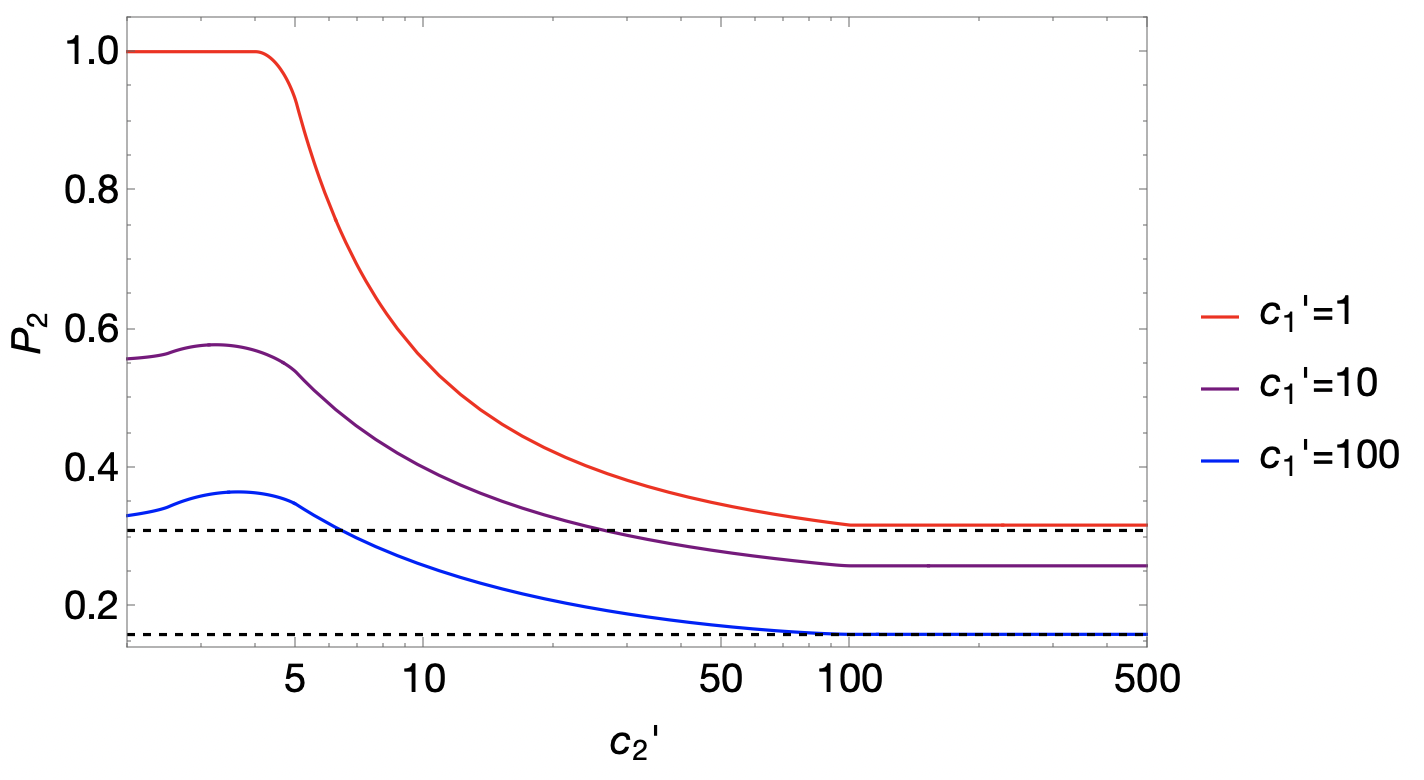
\includegraphics[scale=0.5]{figs/2axion-prob.jpeg}
    \centering
    \caption{Probability of measuring $2.5<\zeta<5$ in the case of two axion as a function of $c_2'$, for different values of $c_1'$. The dashed horizontal lines correspond to the probabilities for 1 and 2 axions as given by Eq. \eqref{eq:bookkeeping-result}: 0.3 and 0.16 respectively.}.
    \label{fig:2axion-prob}
\end{figure}

The behavior of $P_2$ shows that there is a little more nuance, but the result that an axion contributes to the anthropic measure once $c'>\zeta_\text{upper}$ holds true. We see that if $c_1'\ll\zeta_\text{upper}$ and $c_2'>\zeta_\text{upper}$ (see red line for larger $c_2'$ in Fig. \ref{fig:2axion-prob}), the the first axion does not contribute while the second one does, and thus we recover the $P=0.3$ probability from the 1-axion scenario. The same is true if $c_1'>\zeta_\text{upper}$ and $c_2'\ll\zeta_\text{upper}$ (Fig. \ref{fig:2axion-prob}, blue line for small $c_2'$). If both $c_1',c_2'>\zeta_\text{upper}$ (Fig. \ref{fig:2axion-prob}, blue line for large $c_2'$), then the two axions contribute to the measure and so the probability is $P=0.16$, in agreement with Eq. \eqref{eq:bookkeeping-result}. There is a weird middle regime (purple line in Fig. \ref{fig:2axion-prob}, as well as region in all three lines where there is a bump), where I am not really sure what's going on yet. 

We have thus seen, in the case of 1 and 2 axions, that the condition that an axion must satisfy to contribute to the anthropic measure is $c'>\zeta_\text{upper}$. Recalling that $c'=c\,f(H)^2$ (with $f(H)$ given in Eq. \eqref{eq:f(H)}), and that $c=(m/H_{eq})^{1/2}(f/M_{pl})^2$ we can write this condition in terms of the physical parameters as:

\begin{equation}
    \label{eq:c-condition}
    \boxed{\left(\frac{m}{H_{eq}}\right)^{1/2}\left(\frac{f}{M_{pl}}\right)^{2}\min{ \Bigl\{ \pi^2,\frac{3H^4}{8\pi^2m^2f^2}\Bigr\}}>\zeta_\text{upper}}
\end{equation}

The takeaway is that if the scale of inflation is low, heavier axions will evade this criterion and therefore will not contribute to the anthropic measure: including them in the theory does not require more fine-tuning. On the other hand, if the scale of inflation is high, these axions will quickly satisfy this condition and require fine-tuning, while lighter axions won't (the words ``lighter" and ``heavier" depend on the values of $H$ and $f$ in each case respectively; this will need to be further investigated).

Note that Eq. \eqref{eq:c-condition} is approximate in that: (1) it assumes that $F(\theta_a)\sim\theta^2$, which is not true if $\theta_a \sim O(1)$, in which case there is a small correction; (2) it approximates the distribution of $\theta_a$ in a low scale inflation scenario to be flat between $\pm \sigma$, instead of treating it fully as $\propto \exp{\left(-V(\theta_a)/H^4\right)}$; and (3) it only accounts for regimes where $H<\Lambda$ or $H>\Lambda$, and glosses over the $H\sim\Lambda$ regime.

\begin{figure}[h]
    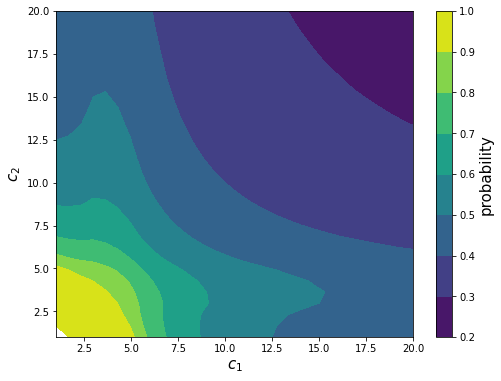
\includegraphics[scale=0.6]{figs/2axion-contour.png}
    \centering
    \caption{Contour plot for the probability shown in Fig. \ref{fig:2axion-prob} as a function of $c_1$ and $c_2$ (numerically plotted, not amazing resolution and only up to $c=20$)}.
    \label{fig:2axion-contour}
\end{figure}

\subsubsection{Geometric interpretation}
\label{subsubsec:geom-interpret}
The challenge of computing the integrals in Eq. \eqref{eq:general-prob} comes from the bounds of integration: the integrand is integrated over each angle $\theta_a$ from $-1$ to $1$, but the integrand is only nonzero for $2.5<\sum_a c_a\theta_a^2<b$, where $b=5$ for the numerator in Eq. \eqref{eq:general-prob} and $b=100$ in the normalization.

To understand what this region of integration looks like, let's go back to the case of 2 axions. In the 2-dimensional space defined by the variables $\theta_1$ and $\theta_2$, the area over which the two dimensional integral in Eq. \eqref{eq:general-prob} is to be computed corresponds to that of an elliptical ring (the $2.5<c_1\theta_1^2+c_2\theta_2^2<b$ constraint), cut off by a square of side length 2 (the bounds of integration for each angle). If $c_1>c_2$, the semi-major axis of the inner (outer) ellipse is determined by $2.5/c_1$ ($b/c_1$), while the semi-minor axis of the inner (outer) ellipse is given by $2.5/c_2$ ($b/c_2$). The values of $c_1$ and $c_2$ therefore determine the size of the elliptical ring. This area is illustrated in Fig. \ref{fig:2d-integration-area} for a few choices of $c_1$ and $c_2$.

\begin{figure}[h]
    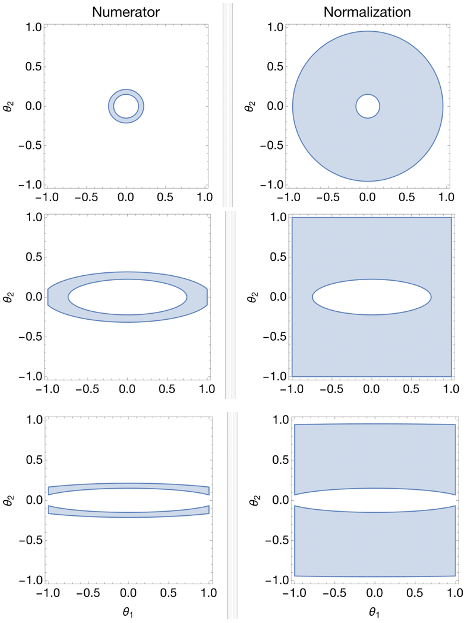
\includegraphics[scale=0.5]{figs/ellipses.png}
    \centering
    \caption{(this is a bad figure but just for illustrative purposes for now) First row corresponds to $c_1 = 100, c_2=110$; middle row is $c_1 = 4.5, c_2=50$; bottom row is $c_1 = 2, c_2=110$.}
    \label{fig:2d-integration-area}
\end{figure}


While ultimately each point on the integration region will be weighted by the integrand (points away from the origin will carry less weight), having a sense of how this region is altered as $c_1$ and $c_2$ vary is important in understanding the resulting integral. There are a few regimes of interest that we will see can be mapped onto the behavior that appears in Fig. \ref{fig:2axion-prob}. These depend on regions of integration of both the numerator and normalization integrals. These are:
\begin{enumerate}
    \item \textbf{when the elliptical ring is fully inside the square in both integrals}: This happens when either $c_1$ or $c_2 > 100$. This is set by the value of semi-major(minor) axes needed for the ellipses to fit inside the square in both integrals. This case corresponds to the case where the axions are heavy enough that they contribute to the anthropic measure, i.e. the result from \cite{exploring-string-axiverse} given in Eq. \eqref{eq:bookkeeping-result}. The result of the integrations is independent of the $c$'s, since the dependence cancels out in numerator and the normalizaiton
    \item \textbf{when the outer edge of the ellipitcal ring touches the square in the numerator integral}: This happens when the semi-major axis of the outer ellipse is equal to 1, i.e. when $c_1$ (or $c_2$) $=5$. This corresponds to the edge of the bumps in Fig. \ref{fig:2axion-prob}. As $c$ gets smaller, the ellipses get more elongated and the area enclosed in the elliptical ring grows. When $c=5$, this is still the case, but at some point as the ellipses start to exit the square, the rate at which the area grows becomes matched and eventually overtaken by the rate at which area exits the square boundary. This explains the bump behavior.
    \item \textbf{when the inner edge of the elliptical ring touches the square in the numerator integral}: This happens when the semi-major axis of the inner ellipse is equal to 1, i.e. when $c_1$ (or $c_2$) $=2.5$. As $c$ gets smaller after this, the region of integration corresponds to two separate curved bands; as the ellipses get streched out futher and further, they asymptotically get closer to looking like two flat rectangles. At this point, the axion with this small value of $c$ is almost ``decoupled" and irrelevant to the anthropic measure (although not quite, since there is still some curvature to the band for a while). This explains the asymptotic behavior of the curves in Fig. \ref{fig:2axion-prob} at small $c_2$, rather than the exactly flat behavior when $c_2>100$.
\end{enumerate}

\subsection{$n$ axions}
\subsubsection{Thresholds}
Following the discussion in Section \ref{subsubsec:geom-interpret}, we can understand the interesting threshold regimes of Eq. \eqref{eq:general-prob} for $n$ axions. In $n$-dimensions, the elliptical ring inside the square from the 2-dimensional case becomes an hyperellipsoidal (?) shell within a hypercube. ... \\
Range of intermediate c's that we don't understand

\subsubsection{Probability for $n$ axions with equal $c$'s}
The easiest case to consider for $n$ axions is when all of them have the same $c$. In this case, the integrals in Eq. \eqref{eq:general-prob} reduce to 1-dimensional integrals in hyperspherical coordinates, over the radial coordinate ($r\equiv\sum_a\theta_a^2$):

\begin{equation}
    \label{eq:nAxions-equalC}
         P = \mathcal{N'}^{-1} \int_{0}^1 \frac{r^{n-1} dr}{1+c r^2}\Theta(c r^2-2.5)\Theta(5-c r^2)
\end{equation}

Fig. \ref{fig:n-prob-equalC} shows the result of Eq. \eqref{eq:nAxions-equalC} for chosen values of $n$. The behavior is as expected: as the number of axions increases, the probability drops to zero more and more quickly. The two regimes to notice are firstly, when $c<5$, the axions are all light enough that we can ignore them in the anthropic measure, and secondly, when $c>100$, the probability reaches its $c$-independent value, as calculated in \cite{exploring-string-axiverse}. These two thersholds are valid for all values of $n$ (the second thershold when $c>100$ is not so obvious for larger $n$, but I checked this numerically.)

More quantitatively, for the values $5<c\leq 100$, Eq. \eqref{eq:nAxions-equalC} evaluates to the following:

\begin{equation}
    P = \frac{B(-2/5;1-n/2,0)-B(-1/5;1-n/2,0)}{B(-2/5;1-n/2,0)-B(-1/c;1-n/2,0)}
\end{equation}

\noindent where $B(x;a,b)$ is the incomplete beta function: $\int_0^x t^{a-1}(1-t)^{b-1} dt$.
\emph{Also thought about perturbing away from equal c's to get slightly different c's for each axions; finding probability for scenarios where one group of axions has 1 value of c and the remaining have another value.}

\begin{figure}[h]
    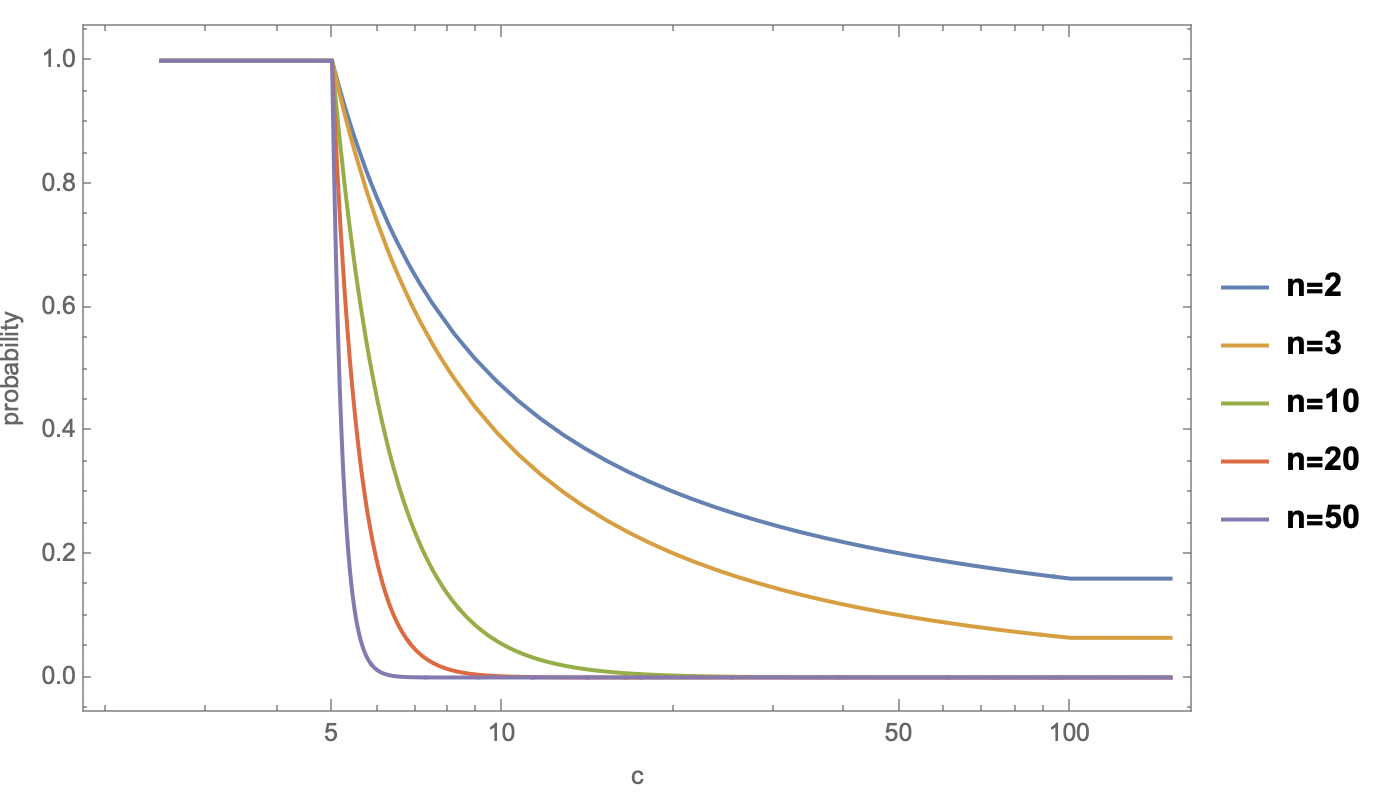
\includegraphics[scale=0.45]{figs/naxions-equalC.png}
    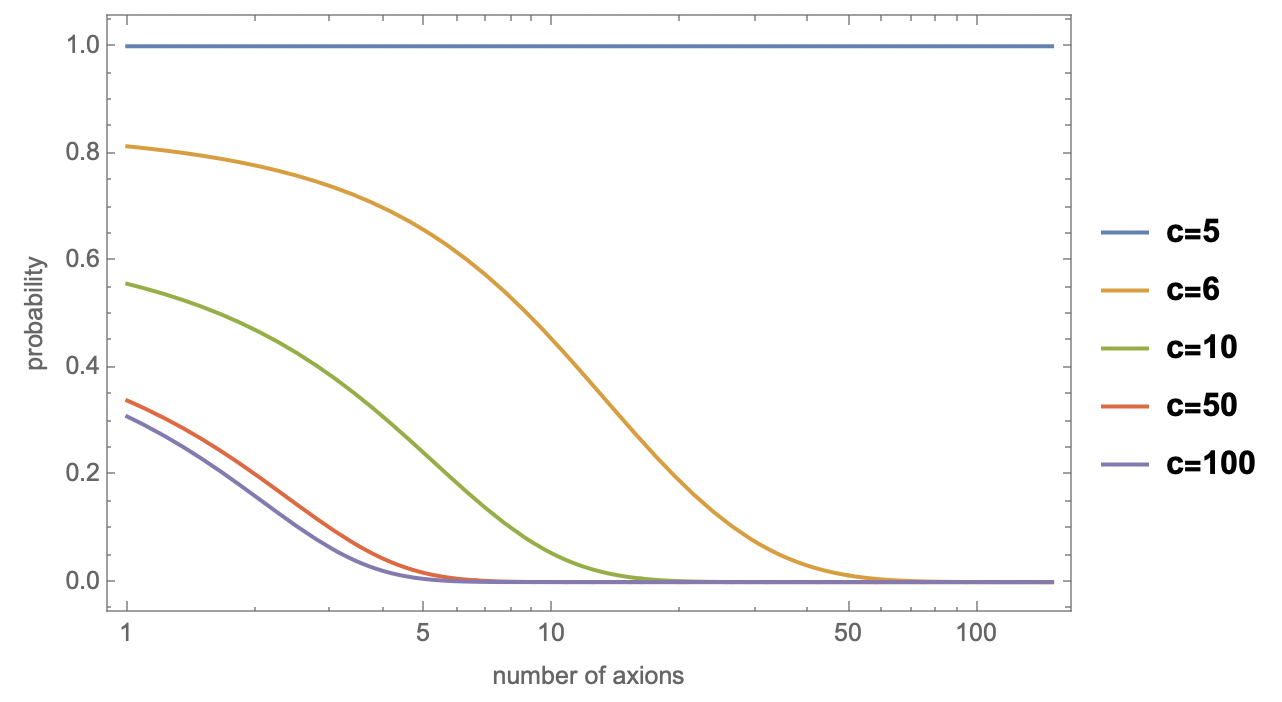
\includegraphics[scale=0.5]{figs/naxions-equalC-vsN.png}
    \centering
    \caption{Top: Eq. \eqref{eq:general-prob} for different choices of $n$ axions, where all axions have the same $c$. Bottom: Probability versus number of axions $n$, for chosen fixed values of $c$. For all values of $c<5$, the probability curve lies on top of the blue curve, and for all values of $c>100$, the curve lies on top of the purple curve.}
    \label{fig:n-prob-equalC}
\end{figure}

\break

\begin{figure}[h]
    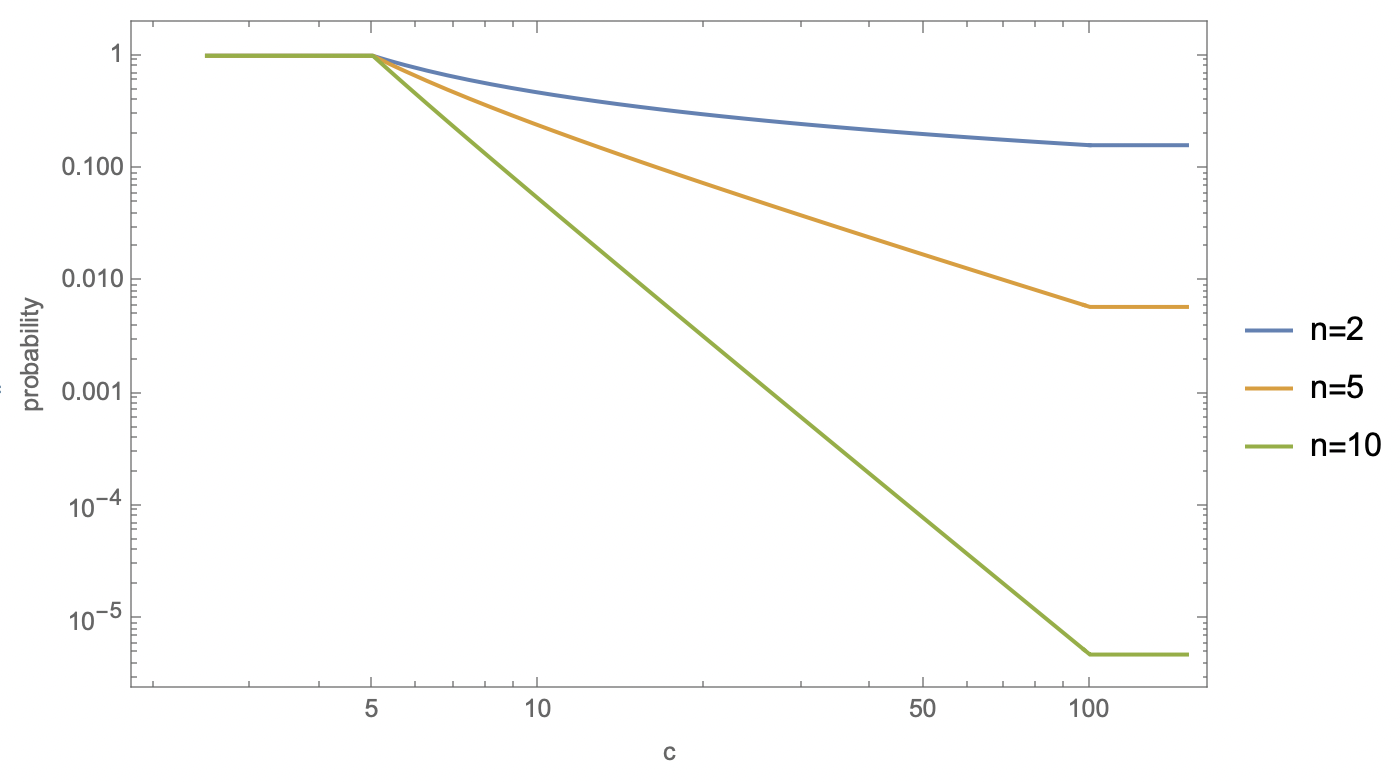
\includegraphics[scale=0.45]{figs/naxions-equalC-loglog1.png}
    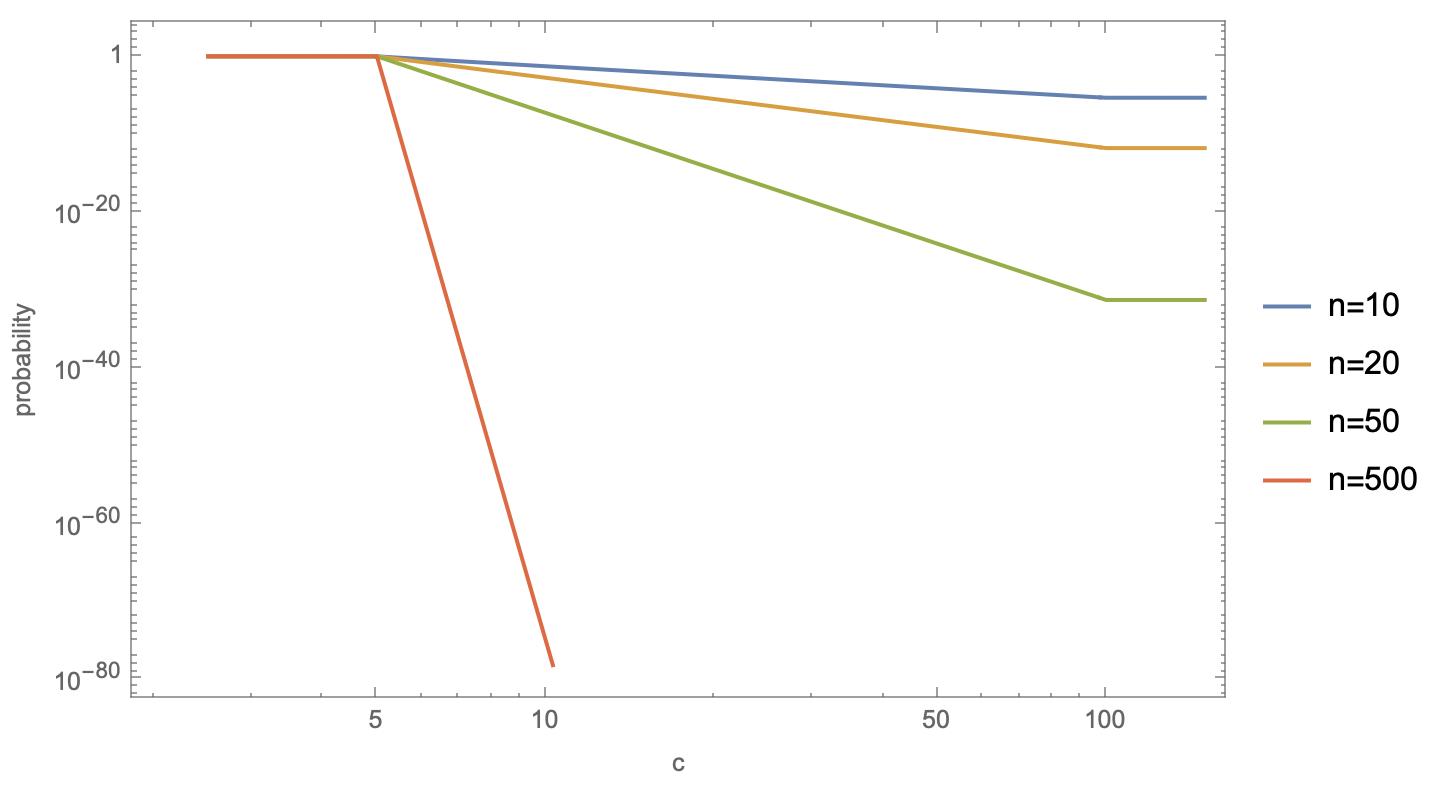
\includegraphics[scale=0.45]{figs/naxions-equalC-loglog2.png}
    \centering
    \caption{Same as Fig. \ref{fig:n-prob-equalC} (probability vs. common $c$) but on a log-log scale, and for larger values of $n$.}
    \label{fig:n-prob-equalC-loglog}
\end{figure}

\subsubsection{Probability for $n$ axions in two $c$ regimes}

Because the anthropic probability has these two regimes when $c<5$ and when $c>100$, we can neglect the regime where $5<c<100$ which we do not understand very well, and simplify the integrals in Eq. \eqref{eq:general-prob} as follows. If we are interested in $n$ axions, and a fraction $\mathcal{F}$ of them have $c>100$, while a fraction $1-\mathcal{F}$ of them have $c<5$, then we can separate the integration variables into two sets, such that the heavy ones can be written in spherical coordinates with $r_1 \equiv \sum_{i=1}^{\mathcal{F}n} \theta_i^2$ and the light ones as $r_2 \equiv \sum_{i=\mathcal{F}n+1}^{n} \theta_i^2$. Then Eq. \eqref{eq:general-prob} can be written:

\begin{equation}
    \label{eq:2groups-naxions}
    P = \mathcal{N}^{-1}\int_{0}^1\int_{0}^1 \frac{r_1^{\mathcal{F}n-1} r_2^{(1-\mathcal{F})n-1} dr_1 dr_2}{1+c_{H}r_1^2+c_{L}r_2^2}
    \Theta(2.5<1+c_{H}r_1^2+c_{L}r_2^2<5)
\end{equation}

\noindent where the normalization $\mathcal{N}$ is the same integral but with the constraint $2.5<1+c_{H}r_1^2+c_{L}r_2^2<100$. This integral can be computed numerically and its result is shown in Fig. \ref{fig:n-axions-2groups.png} below for $n=4$ and a few choices of $\mathcal{F}$.

\begin{figure}[h]
    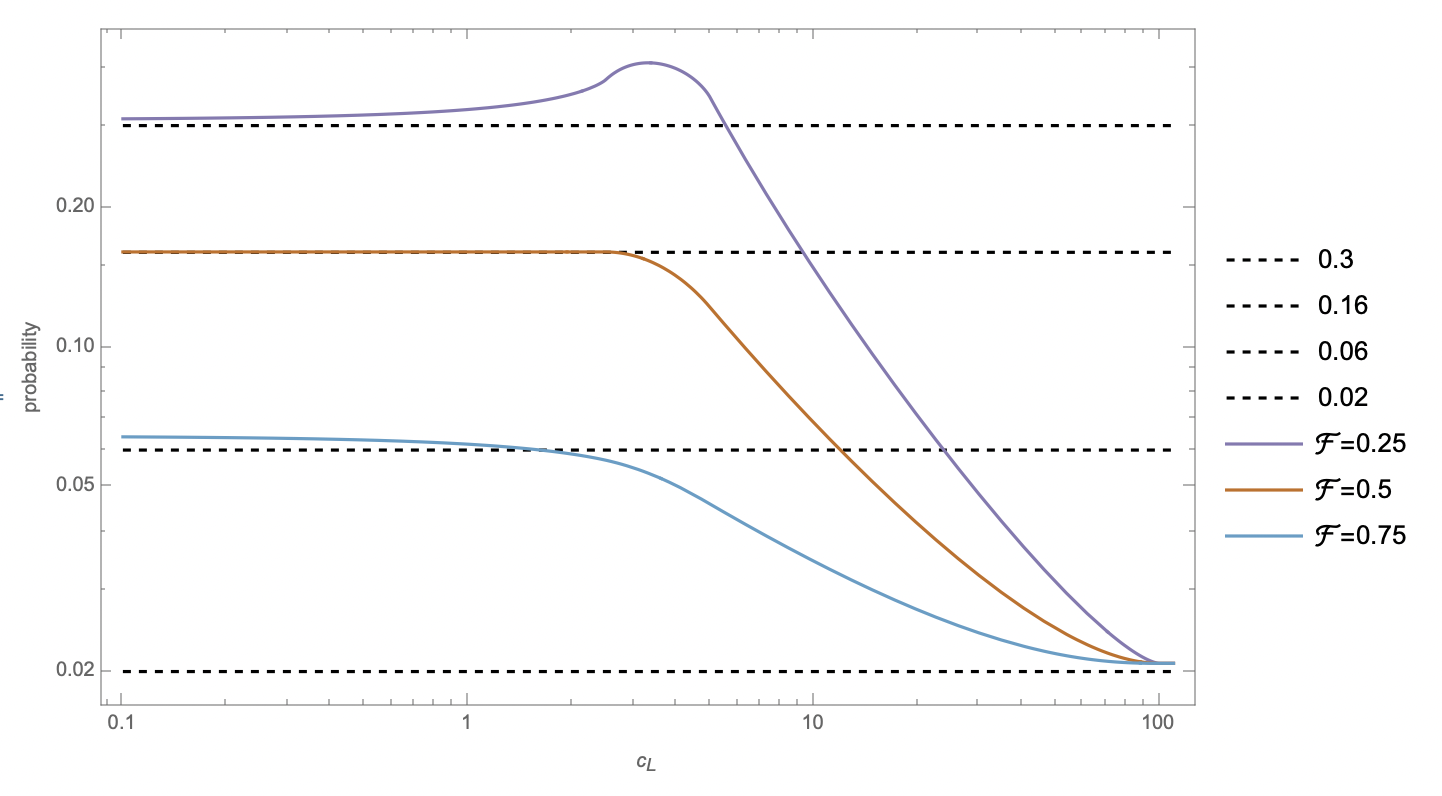
\includegraphics[scale=0.55]{figs/n-axions-2groups2.png}
    \centering
    \caption{The result of Eq. \eqref{eq:2groups-naxions} fo $n=4$ and $c_H=100$. The dashed lines show the probabilities for 1,2,3, and 4 axions contributing to the anthropic measure. The x-axis is $c_L$ and the fraction of axions that have this value of $c$ is given by $1-\mathcal{F}$. If $c_L>100$, we see the probability is equal to that of 4 axions for all choices of $\mathcal{F}$, while if $c_L<5$, the probabiltiy approaches that for $\mathcal{F}n$ axions for each chosen value of $\mathcal{F}$ and $n=4$.}
    \label{fig:n-axions-2groups.png}
\end{figure}

We can therefore conclude that for all $n$, if an axion is light ($c\lesssim2.5-5$), it will not contribute to the anthropic measure, while if it is heavy ($c>100$), it will.

\subsection{Allowed parts of parameter space}

Eq. \eqref{eq:c-condition} tells us that certain choices of $m, f$ and $H_I$ will lead to an axion contributing to the anthropic probability. The plot below shows the part of parameter space that are allowed by anthropics for a single axion with mass $m$ and decay constant $f$, for different fixed values of $H_I$. The part of parameter space that lies above the lines leads to values of $c>100$ and thus corresponds to parts of parameter space where the axion contributes to the anthropic measure.

\begin{figure}[h]
    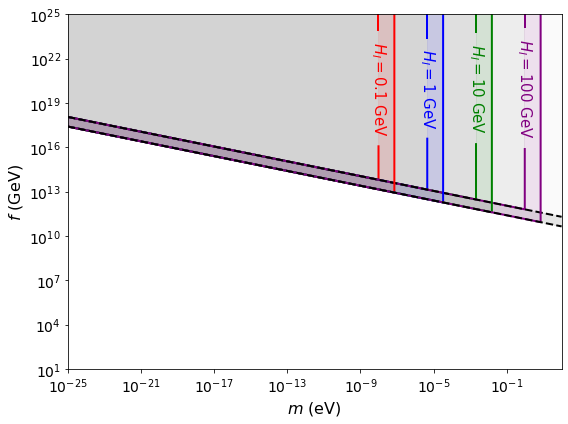
\includegraphics[scale=0.6]{figs/f-vs-m-anthropic.png}
    \centering
    \caption{The grey shaded regions show the parts of parameter space that contribute to the anthropic probability, delimited by different colored lines corresponding to different choices of $H_I$. The white region corresponds to choices of axion parameters that do not contribute to the anthropic probability. The colorful bands correspond to the range $5<c<100$ over which we do not really understand the contribution to the anthropic measure.}
    \label{fig:f-vs-a}
\end{figure}

The black dashed line goes like $m^{-1/4}$ and corresponds to Eq. \eqref{eq:c-condition} when $\min{ \Bigl\{ \pi^2,\frac{3H^4}{8\pi^2m^2f^2}\Bigr\}} = \pi^2$, while the vertical lines correspond to the second case (which, notice in Eq. \eqref{eq:c-condition}, leads to a value of $c$ that does not depend on $f$). The grey shaded region corresponds to the ``anthropic region" for a given choice of $H_I$– the part of parameter space in which an axion would contribute to the anthropic measure. As the scale of inflation decreases, the anthropic region gets smaller since for low $H_I$, smaller misalignment angles are allowed, meaning that heavier axions can evade the requirement for contributing to the anthropic measure. The colorful shaded regions correspond to the intermediate range of $c$'s for which we do not fully understand the probability distribution (i.e. $5<c<100$). The white region of the plot correspond to choices of $(m,f)$ which do not contribute to the anthropic measure.

\break
\color{red}\noindent \textbf{Things to do:}
\begin{enumerate}
    \item could include correction to the energy density from cosine potential in the probability calc
    \item \st{what happens below $c=\zeta_\text{upper}$?}
    \item \st{and related to the previous point, what is the bump? what does it looks like with more axions?}
    \item \st{visualize}/better understand the parts of parameter space that are viable via anthropics using Eq. \eqref{eq:c-condition}
    \item keep in mind dependence of results on choice of measure (causal diamond vs others?)
    \item how does Eq. \eqref{eq:c-condition} depend on number of axions?
    \item fig 3 but same quantities plotted as fig 2 for easier comparison
\end{enumerate}\color{black}

\section{Energy densities of 2 axions}

David's simulations suggest that when there are couplings between many axions, the relic abundance in each axion no longer follow the expected $m^{1/2}$ scaling that we expect from misalignment (see. Fig. \ref{fig:e-density-uncoupled} vs. Fig. \ref{fig:e-density-coupled}).

\begin{figure}[h]
    \centering
    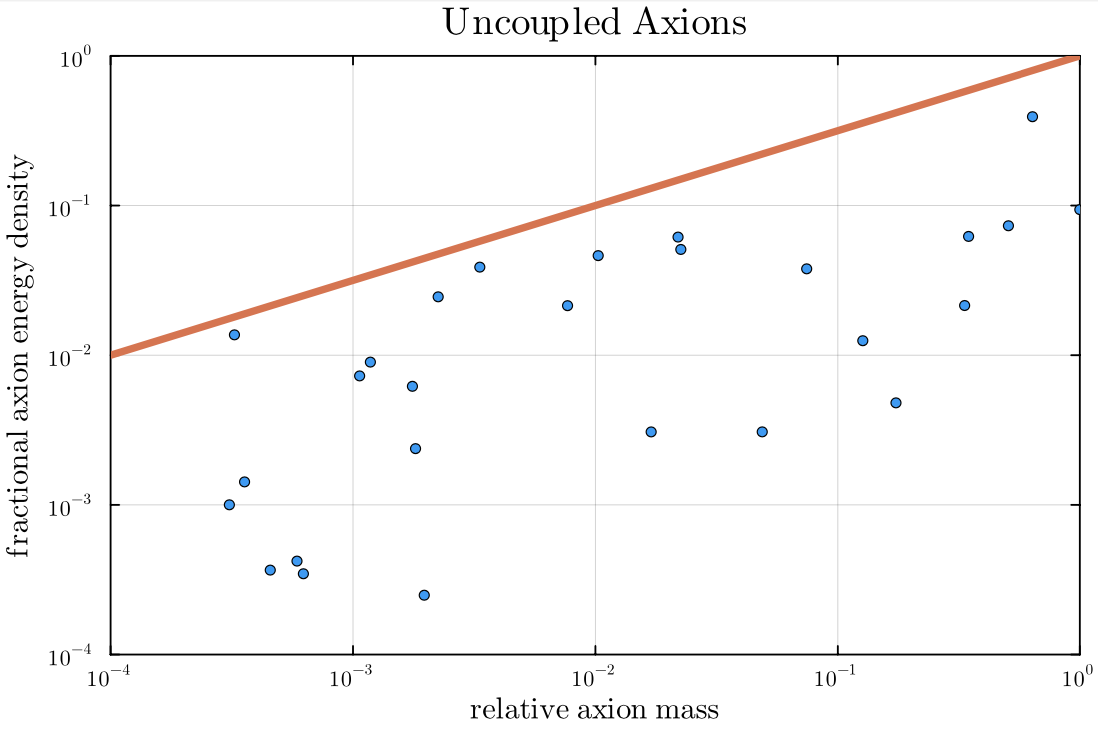
\includegraphics[width=0.9\linewidth]{figs/Uncoupled_Axions.png}
    \caption{Energy density of 30 uncoupled axions. Each point corresponds to an axion of mass given by the x-axis (normalized to the heaviest axion) and energy density given by the y-axis (normalized by the total energy density).}
    \label{fig:e-density-uncoupled}
\end{figure}
\begin{figure}[h]
    \centering
    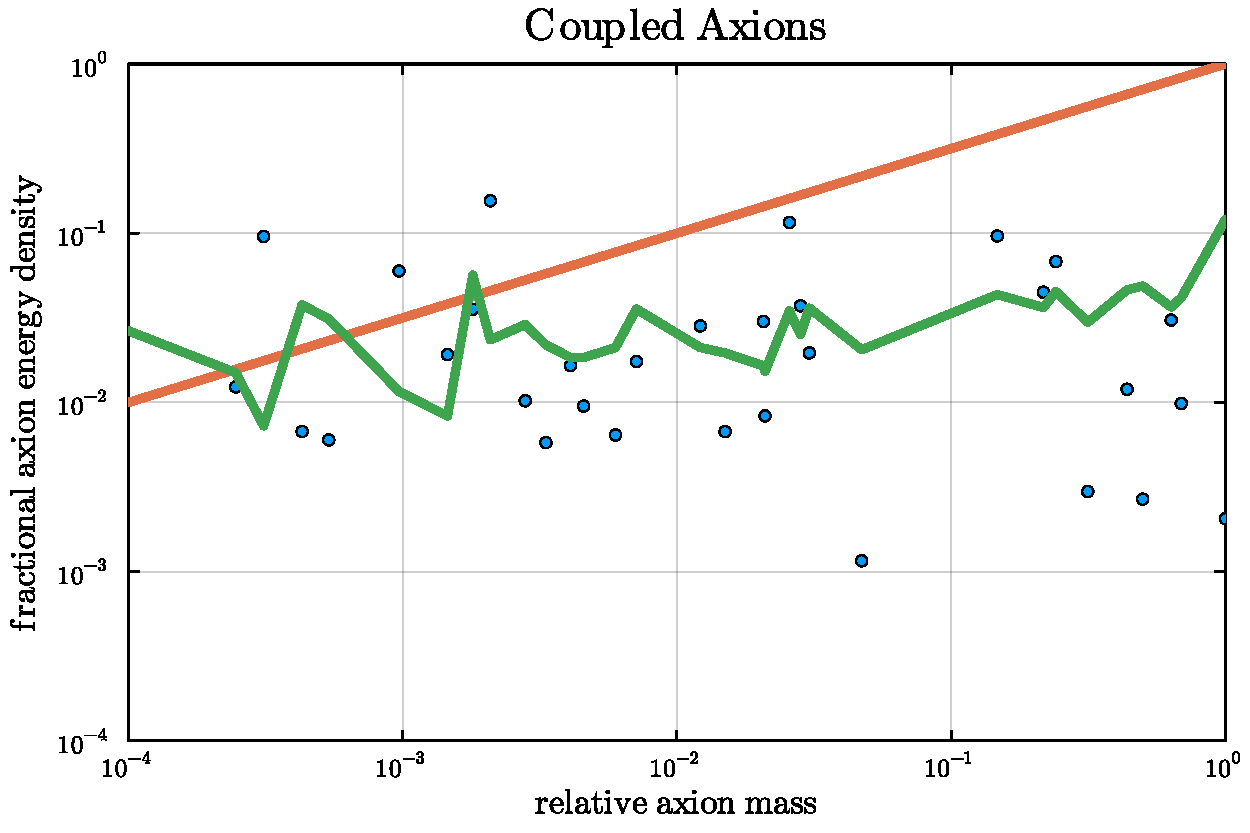
\includegraphics[width=0.9\linewidth]{figs/Coupled_Axions_With_GS.pdf}
    \caption{Energy density of 30 coupled axions measured from one simulation (blue dots). Same axes as above. It appears that the $m^{1/2}$ scaling (red) falls apart when interactions are present. The green line is the expected energy density using the decay constants inferred from the Gram-Schmidt basis decay constants. While more data is required to be able to say anything definitive, $\chi$-by-eye suggests that the green prediction does not fully capture the trend in the blue data.}
    \label{fig:e-density-coupled}
\end{figure}

Our goal is to determine if there really is energy redistribution among interacting axions and if so, what this process physically coresponds to. To do this, we'll start with two axions.

\subsection{Gram–Schmidtification procedure}
\label{subsec:GS-2-axions}
Consider a theory of two interacting axions $\varphi_1/f_1\equiv\theta_1$ and $\varphi_2/f_2\equiv\theta_2$ with a Lagrangian of the following form:

\begin{equation}
    \label{eq:pre-GS-potential}
    \mathcal{L} = \frac{1}{2}\partial_\mu\theta_1 \partial^\mu\theta_1  + \frac{1}{2}\partial_\mu\theta_2 \partial^\mu\theta_2  + \Lambda_{b}\cos{(a\theta_1+b\theta_2)}+\Lambda_{s}\cos{(c\theta_1+d\theta_2))}
\end{equation}

\noindent where we can assume $\Lambda_b>\Lambda_s$ and have set $f_1 = f_2 = 1$ for now. The mixing matrix between the two fields can be written as follows:
\begin{equation}
A \equiv
    \begin{pmatrix}
    a & b\\
    c & d
    \end{pmatrix}
\end{equation}

Following the Gram-Schmidtificaiton (GS) procedure, we want to perform a change of basis in order to rewrite this  matrix as a lower triangular one, call it $T$. In other words, we are looking to redefine the fields in the above Lagrangian, so that the first cosine term contains only one redefined field, say $\phi_1$, while the second contains a linear combination of  $\phi_1$ and the second redefined field, $\phi_2$:

\begin{equation}
    \label{eq:triang}
    \begin{cases}
        a\theta_1+b\theta_2 = t_{11} \phi_1 \\ 
        c\theta_1+d\theta_2 = t_{21} \phi_1 + t_{22} \phi_2
    \end{cases} \,\,\,\,\,
    \Leftrightarrow \,\,\,\,\,
    A \begin{pmatrix}
        \theta_1 \\
        \theta_2
    \end{pmatrix}
    = 
    \begin{pmatrix}
        t_{11} & 0 \\
        t_{21} &t_{22} 
    \end{pmatrix} 
    \begin{pmatrix}
        \phi_1 \\
        \phi_2
    \end{pmatrix}
\end{equation}

We want to choose the $d_{ij}$ so that the kinetic terms remain in canonical form after redefinition, so we will impose  $\frac{1}{2}\partial_\mu\theta_i \partial^\mu\theta_i = \frac{1}{2}\partial_\mu\phi_i \partial^\mu\phi_i $ and no cross terms. Dropping factors of $1/2$ and derivatives for less cumbersome computation, we impose $\theta_i^2 = \phi^2_i$. Using Eq. \eqref{eq:triang}, we write $\theta_1$ and $\theta_2$ in terms of the redefined fields:

\begin{equation}
    \begin{pmatrix}
        \theta_1 \\
        \theta_2
    \end{pmatrix}
    = 
   A^{-1} T 
    \begin{pmatrix}
        \phi_1 \\
        \phi_2
    \end{pmatrix}
\end{equation}

\noindent Using the matrices $A$ and $T$ as defined above, and then perform an inner product of this vector with itself to find:

\begin{align*}
     \label{eq:dotprod}
    \theta_1^2+\theta_2^2 = \frac{1}{(\det{A})^2} \big[ 
    \phi_1^2 \left(t_{21}^2 \left(a^2+b^2\right)-2 t_{11}t_{21} (a c+b d)+t_{11}^2 \left(c^2+d^2\right)\right) \\
    + 2 t_{22} \phi _2 \phi _1 \left(t_{21}\left(a^2+b^2\right)-t_{11} (a c+b d)\right)+t_{22}^2 \phi _2^2 \left(a^2+b^2\right)
    \big]
\end{align*}

The condition from the canonical kinetic terms means that we must impose:

\begin{equation}
    \label{eq:constraints}
    \begin{cases}
        \text{coefficient of }\phi_1^2 = (\det{A})^{-2}\big((d-bx)^2+(ax-c)^2\big)= 1 \\
        \text{coefficient of }\phi_1\phi_2 = (\det{A})^{-2}\big(2(d-bx)by-2(ax-c)ay\big)= 0 \\
        \text{coefficient of }\phi_2^2 = (\det{A})^{-2}y^2(b^2+a^2) =1 \\
    \end{cases}
\end{equation}

Solving for $t_{ij}$, we find:

\begin{equation}
    \begin{cases}
        t_{11} = \sqrt{a^2+b^2} \\
        t_{21} = \frac{ca+db}{(\det{A})^2} \\
        t_{22} = \pm \frac{\det{A}}{\sqrt{a^2+b^2}}
    \end{cases}
\end{equation}

Thus, the Lagrangian is:

\begin{align*}
   \mathcal{L} = &  \frac{1}{2}\partial_\mu\phi_1\partial^\mu\phi_1+\frac{1}{2}\partial_\mu\phi_2\partial^\mu\phi_2+\Lambda_b\cos{(\sqrt{a^2+b^2}\phi_1)}+\Lambda_s\cos{\bigg(\frac{(ca+db)\phi_1+\det{A}\phi_2}{\sqrt{a^2+b^2}}\bigg)} \\
   \sim & \frac{1}{2}\partial_\mu\phi_1\partial^\mu\phi_1+\frac{1}{2}\partial_\mu\phi_2\partial^\mu\phi_2+\Lambda_b\cos{(\sqrt{a^2+b^2}\phi_1)}+\Lambda_s\cos{\bigg(\frac{\det{A}}{\sqrt{a^2+b^2}\phi_2}\bigg)}
\end{align*}

Because $\Lambda_b>\Lambda_s$, $\phi_1$ will receive the significant part of its dynamics from the first cosine term and so we can view this as the Lagrangian for two decoupled axions, $\phi_1$ and $\phi_2$, each in their own cosine potential. The fields have a mass hierarchy set by $\Lambda_b>\Lambda_s$ and have decay constants rescaled from those of the original theory as follows:
\begin{equation}
    \label{eq:decay-consts-GS}
    \begin{cases}
        f_1 \rightarrow f_1/\sqrt{a^2+b^2)} \\
        f_2 \rightarrow f_2(a^2+b^2)/\det{A}
    \end{cases}
\end{equation}

\subsection{From interacting to ``uncoupled" axions: relative energy densities}
\label{subsec:GS-powerlaw}
Now consider the slope, $\gamma$, in the $\log{(\rho_2/\rho_1)}$ vs. $\log{(m_2/m_1)}$ plane, where $\rho_{1(2)}\sim m_{1(2)}^{1/2}(f_{1(2)}\theta_{i,1(2)})^2$ is the energy density in the decoupled fields $\phi_{1(2)}$, and $m_{1(2)}$ is its mass. For uniformly distributed misalignment angles, $\phi_{i,1(2)}$, the expectation for this power law is given by:

\begin{equation}
    \label{eq:power-law}
    \langle \gamma \rangle = \frac{\log{(m_2^{1/2}f_2^2)}-\log{(m_1^{1/2}f_1^2)}}{\log{(m_2/m_1)}}
\end{equation}

After the GS procedure, we send the decay constants to their rescaled values as given in Eq. \eqref{eq:decay-consts-GS} and we find that we can write:

\begin{equation}
    \label{eq:GS-exp-gamma}
    \langle \gamma \rangle = \frac{\log{(F(m_2/m_1)^{1/2})}}{\log{(m_2/m_1)}}
\end{equation}
 
\noindent where $F \equiv ((a^2+b^2)/\det{A})^2$ and we have set the decay constants $f_1=f_2=1$. In our problem, the mixing coefficients $\{a,b,c,d\}$ are each chosen from $\{-1,0,1\}$ with equal probability. We would like to compute an average value of the power law, given that our potential is chosen at random in this manner. We find that there are only four possible values for $F$: 0, undefined,1,1/4. The cases where $F=0$ or $F$ is undefined are not physically interesting as they correspond to cases where either the linear combinations in the cosine terms are linearly dependent, or where too many of these coefficients are zero, and so the fields may not appear at all in the potential, or may not be mixed. If these values of $F$ are drawn, then we redraw mixing coefficients (if the potential had more cosine terms, this would be equivalent to moving to the cosine with the next largest $\Lambda$). We can do this as many times as it takes to get $F=1$ or $F=1/4$, which corresponds to a Markov chain process, and we can calculate the probability of ending up in these configurations by constructing a transition matrix, where the rows correspond to the incoming state, and the columns correspond to the outgoing state. As an example, I will work out the problem for the configuration/potential-choosing method outlined above. 

There are 81 possible choices for the pairs $(a,b)$ and $(c,d)$. Out of those 81, 24 correspond to cases where $F=0$, 9 to $F= \text{ undefined}$, 32 to $F=1$ and 16 to $F=1/4$. The transition probability matrix is given by:

\begin{equation}
\mathbb{P}=
    \begin{pmatrix}
        24/81 & 9/81 & 32/81 & 18/81 \\
        24/81 & 9/81 & 32/81 & 18/81 \\
        0 & 0 & 1 & 0 \\
        0 & 0 & 0 & 1 \\
    \end{pmatrix}
\end{equation}

\noindent. Here, the choice of basis is such that the probabilities in a row or column correspond to the following order: $(F=0,F=\text{undefined},F=1,F=1/4)$. Notice that the rows add to 1 to conserve probability. The last two rows correspond to the fact that if we chose $a,b,c,$ and $d$ such that $F=1 \text{ or } 1/4$, then we do not re-draw. Probability theory tells us that:

\begin{equation}
    \label{eq:prob-theorem}
    P(X_t=j \, |\,X_0=i) = (\mathbb{P}^t)_{ij}
\end{equation}

\noindent and so we can calculate the probability of starting with either $F=0$ or undefined, and ending in either $F=1 \text{ or } 1/4$ by looking at the appropriate entries of some high power of $\mathbb{P}$, which will end up converging to something close to:

\begin{equation}
        \begin{pmatrix}
        0 & 0 & 2/3 & 1/3 \\
        0 & 0 & 2/3 & 1/3 \\
        0 & 0 & 1 & 0 \\
        0 & 0 & 0 & 1 \\
    \end{pmatrix}
\end{equation}

\noindent Therefore the overall probability of having either $F=1$ or $F=1/4$ is (this is bad notation, inconsistent with notation in Eq. \eqref{eq:prob-theorem} but anyway)

\begin{align}
    P(F=1) & = \frac{32}{81}+ \frac{2}{3}\frac{24+9}{81} = \frac{54}{81}\\
    P(F=\frac{1}{4}) & = \frac{16}{81}+ \frac{1}{3}\frac{24+9}{81} = \frac{27}{81}
\end{align}

\noindent where the second terms in the intermediate step of each line correspond to the contribution form choices of $F=0$ or undefined. We can therefore determine the weighted average of $\langle \gamma\rangle$ using Eq. \eqref{eq:GS-exp-gamma} as:

\begin{align*}
    \langle \gamma\rangle_{GS} & = \frac{54}{81}\frac{1}{2} + \frac{27}{81}\frac{\log{[(1/4)(m_2/m_1)^{1/2}]}}{\log{(m_2/m_1)}} \\
    & = \frac{1}{3}+\frac{27}{81}\bigg( \frac{-\log{4} + \frac{1}{2}\log{(m_2/m_1)}}{\log{(m_2/m_1)}}\bigg)
\end{align*}

\begin{equation}
    \label{eq:GS-powerlaw}
    \Rightarrow \langle \gamma\rangle_{GS}  = \frac{1}{2}-\frac{1}{3}\frac{\log{4}}{\log{(m_2/m_1)}}
\end{equation}

\subsection{Comparing with simulation data}

Consider again the most general potential for two interacting axions:

\begin{equation}
    \label{eq:gen-pot-2axions}
    \mathcal{L} = \frac{1}{2}\partial_\mu\theta_i\partial^\mu\theta_i-\left[\Lambda_1^4\big(1-\cos{(n_{11}\theta_1+n_{12}\theta_2)}\big) +\Lambda_2^4\big(1-\cos{(n_{21}\theta_1+n_{22}\theta_2)}\big)\right]
\end{equation}

The below figure shows results from David's simulations: the y-axis shows the power law $\gamma$ as defined in Eq. \eqref{eq:power-law}, for a given mass ratio $1/\log{(m_2/m_1)}$, given on the x-axis. Each point corresponds to a choice of potential, given in Eq. \eqref{eq:gen-pot-2axions}, where the $n_{ij}$'s are chosen at random from $\{-1,0,1\}$ such that each field shows up at least once and each cosine is linearly independent. Each point (i.e. the outcome of a choice of potential) is averaged over 300 initial conditions for the misalignment angles. 

\begin{figure}[h]
    \centering
    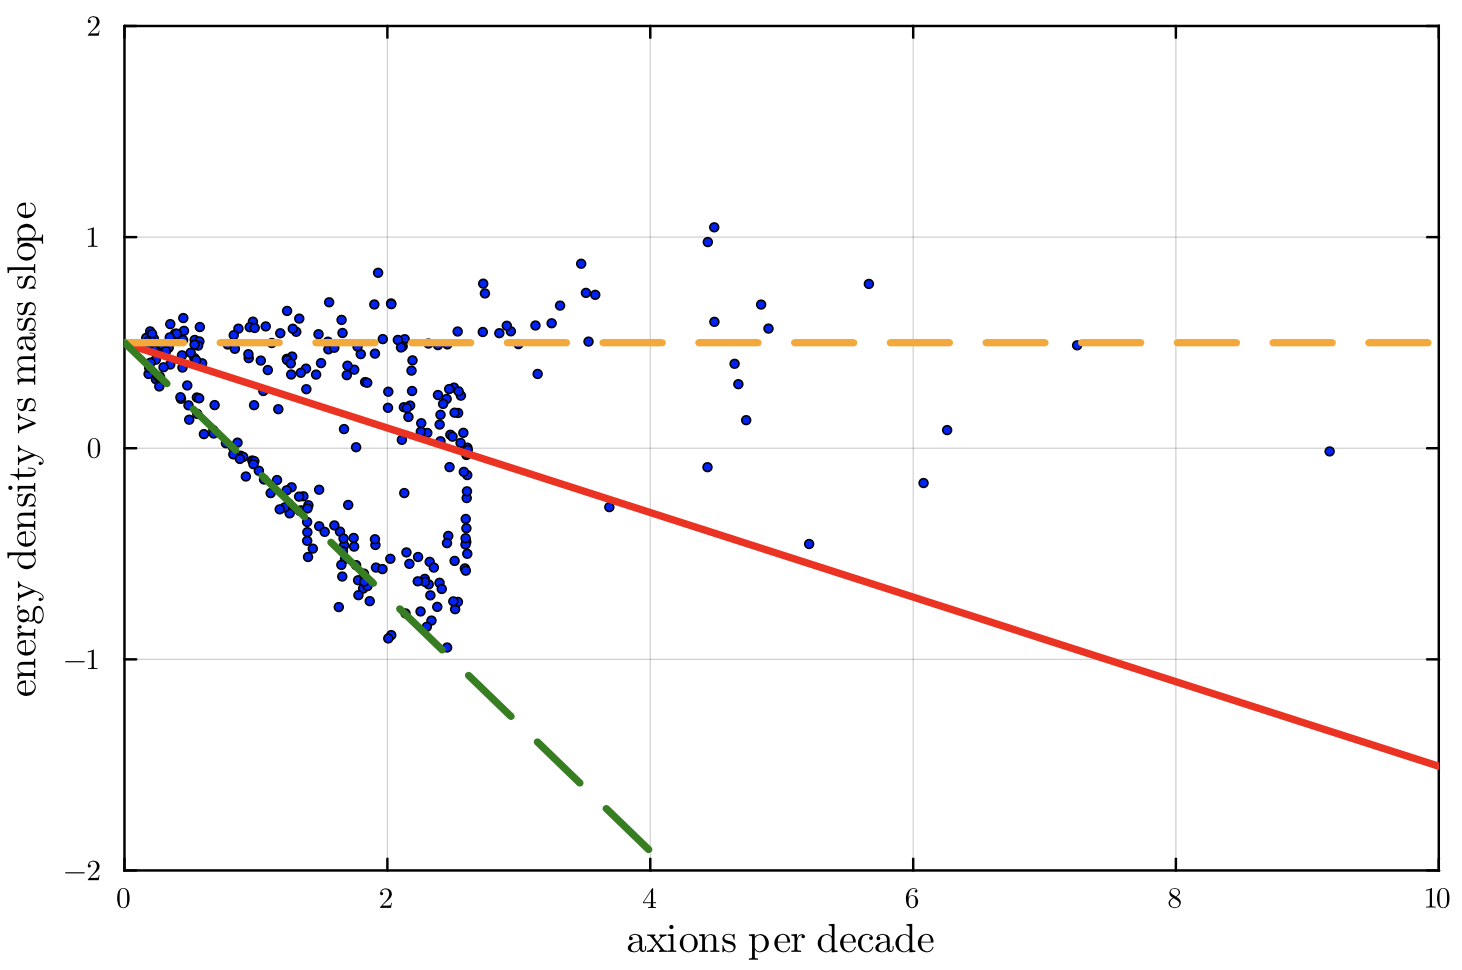
\includegraphics[width=0.9\linewidth]{figs/Slope_vs_ApD.png}
    \caption{The vertical axis shows the power law $\gamma = \log(\rho_2/\rho_1)/\log{(m_2/m_1)}$, and the horizontal axis shows axions per decade of mass, or $1/\log{(m_2/m_1)}$. The red line is the line of best fit, which overlaps with the expression in Eq. \eqref{eq:GS-powerlaw}. The green and orange line correspond to the two cases for the rescaled decay constants discussed in Section \ref{subsec:GS-powerlaw}.}
    \label{fig:2axions-powerlaw-apd}
\end{figure}

In Fig. \ref{fig:2axions-powerlaw-apd}, the red line corresponds to the line of best fit for the data points with axions per decade $<2$. It also overlaps with the analytically calculated average given in Eq. \eqref{eq:GS-powerlaw}. The orange line corresponds to the case where $F=1$, and then green line corresponds to the case where $F=1/4$, as discussed in Section. \ref{subsec:GS-powerlaw}. See below Eq. \eqref{eq:GS-exp-gamma} for the definition of $F$. 

\subsection{GSification generalized to N axions}
\label{subsec:general-GS}

Start with a Lagrangian of the form $\frac12k_{ij}\dot{\theta_i}\dot{\theta_j}+\sum_i\Lambda_i^4(1-\cos{(n_{ij}\theta_j)})$, where we can assume that the $\Lambda_i$ are ordered from largest to smallest. We can generalize the procedure for 2 axions  detailed in Section \ref{subsec:GS-2-axions} to N axions (see David's note for details). We start by redefining the heaviest axion as $\Phi_0 = n_{0i}\theta_i + \delta_0 $ and all other axions as $\Phi_\alpha = \theta_\alpha - c_\alpha\Phi_0 $ where Greek indices start at 1 and Roman start at 0 and the $c_\alpha$ coefficients depend on $n_{ij}$ and $k_{ij}$. Once the Lagrangian is rewritten in terms of these variables and we enforce that the kinetic cross-terms between the 0-th and $\alpha$-th axions vanish, we find that $c_\alpha = - Q_{0\beta}[Q^{-1}]_{\alpha\beta}$ (with $Q$ defined below) and that the 0-th axion is kinetically decoupled from the others with a decay constant:

\begin{equation}
    \label{eq:new-decay-constant}
    \frac{1}{2}f_0^2 = Q_{00} - Q_{0\alpha}Q_{0\beta}[Q^{-1}]_{\alpha\beta}
\end{equation}

\noindent where the matrix Q is a symmetric $(N\times N)$ matrix, given by:

\begin{equation}
    \label{eq:Q}
    Q_{ij} = \begin{pmatrix}
        \frac{k_{00}}{n_{00}^2} & \frac{_{0\alpha}n_{00}-k_{00}n_{0\alpha}}{n_{00}^2} \\
         \frac{k_{0\alpha}n_{00}-k_{00}n_{0\alpha}}{n_{00}^2} & k_{\alpha\beta} - \frac{k_{0\alpha}n_{0\beta}}{n_{00}} - \frac{k_{0\beta}n_{0\alpha}}{n_{00}} + \frac{k_{00} n_{0\alpha}n_{0\beta}}{n_{00}^2}
    \end{pmatrix}
\end{equation}

The remaining $\alpha$-th axions now have kinetic mixing matrix given by $\tilde{k}= Q_{\alpha\beta}$ and potential mixing matrix:

\begin{align}
    \label{eq:remaining-n-matrix}
    \tilde{n}_{\alpha 0} & = \frac{n_{\alpha 0}}{n_{00}} + (n_{\alpha\beta}-\frac{n_{\alpha 0}n_{0 \beta}}{n_{00}})c_\beta\\
    \tilde{n}_{\alpha\beta} & = n_{\alpha\beta} - \frac{n_{\alpha 0}n_{0 \beta}}{n_{00}}
\end{align}

These results can be fully rewritten in terms of matrix operations. If we define the $(N\times N)$ dimensional matrix

\begin{equation}
    S \equiv \begin{pmatrix}
        1/n_{00} & -n_{0\alpha}/n_{00} \\
        0 & \mathbb{1}
    \end{pmatrix}
\end{equation}

\noindent then $Q = S^TkS$ and the above results in Eqs. \eqref{eq:new-decay-constant}, and \eqref{eq:remaining-n-matrix} become:

\begin{align}
    \tilde{n} & = [S^TnS]_{\alpha\beta} \\
    \tilde{k} & = [S^TkS]_{\alpha\beta} \\
    \frac{1}{2}f^2 & = \frac{1}{[Q^{-1}]_{00}}  = (\vec n^T k^{-1} \vec n)^{-1}\label{eq:f-matrix-version}
\end{align}
where $\vec{n} \equiv n_{0i}$.

This procedure is repeated $N$ times until every axion is independent. At each step, after GS-ification of the heaviest remaining field, we set the remaining interaction term between this heaviest axion and all the remaining ones (i.e. the term with coefficient $\tilde{n}_{\alpha 0}$) to zero, as the dynamics of the heaviest axion are primarily determined by its own potential. In this way, the mixing matrices $n$ and $k$ decrease in dimesion by 1 at each step, and the decay constant of the $i$-th axion is given by $\frac{1}{2}(f_{(i)})^2 = 1/[(Q_{(i)})^{-1}]_{00}$, where the lower index denotes the $i$-th axion.

\subsubsection{Understanding scaling of $f$ as a function of $N$}

We can numerically evaluate the $f_{(i)}$'s for some random choice of a symmetric, positive definite $k_{ij}$ matrix and integer $n_{ij}$ matrix. The plot below in Fig. \ref{fig:f-vs-axions} shows the decay constant of the $i$-th axion on the vertical axis after each step of GS-ification, against $i$ on the horizontal axis, which indexes the axions from heaviest to lightest. In this example, the initial $k_{ij}$ matrix is generated by first generating a diagonal $N\times N$ matrix with random entries between $[0,1)$ (to ensure the matrix is positive definite), and then transforming it by a random element of $SO(N)$. The initial $n_{ij}$ matrix is generated by randomly assigning an integer between $[-10,10]$ to each entry.

The general behavior of the curve is in agreement with the 2-axion result, where the lighter axion had an enhanced decay constant after GS-ification, while the heavier axion had a supressed decay constant.

\begin{figure}[h]
    \centering
    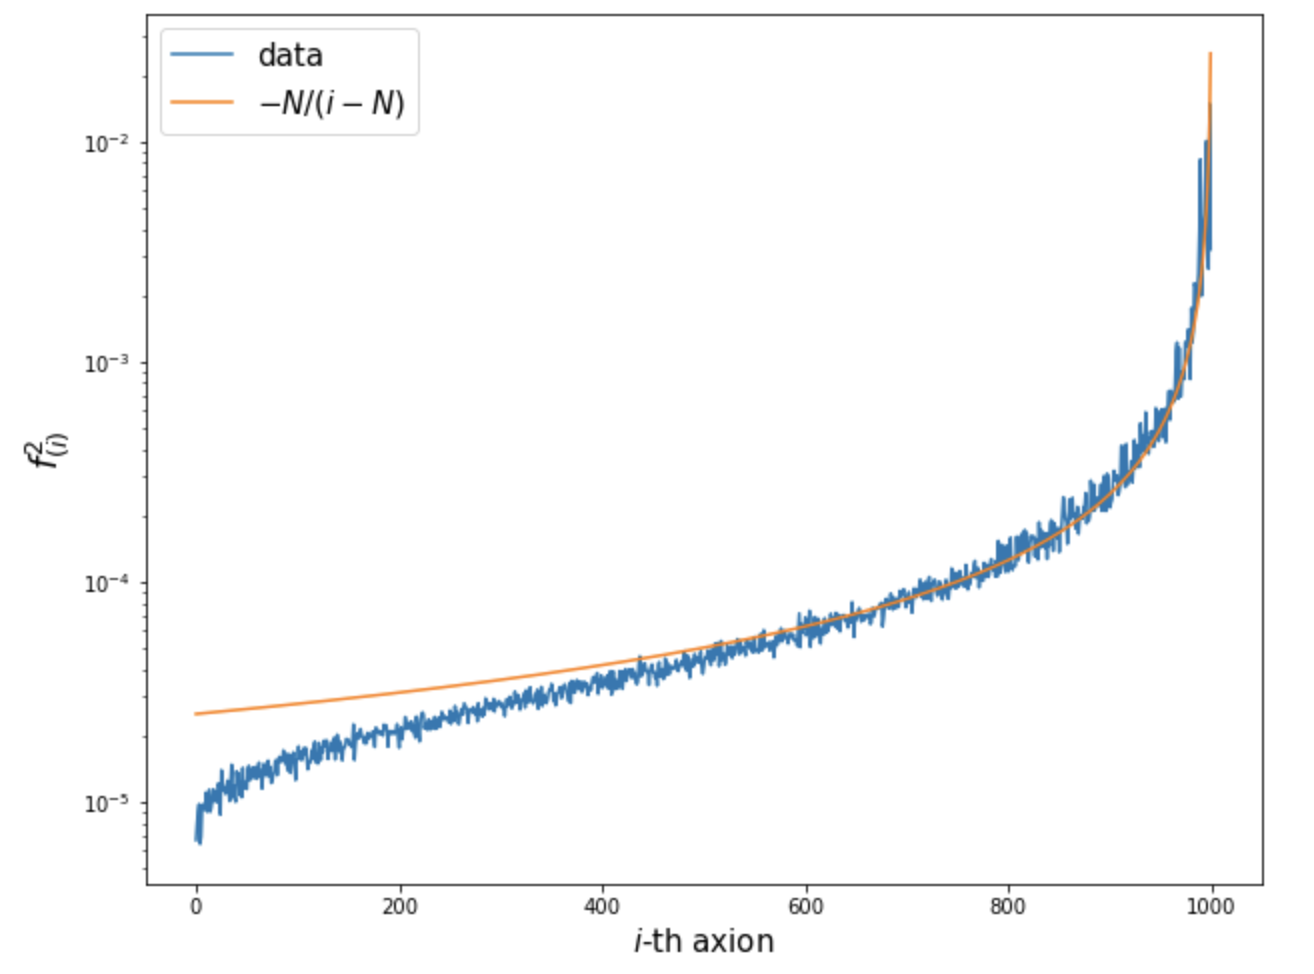
\includegraphics[width=0.9\linewidth]{figs/f-vs-axions.png}
    \caption{The blue curve shows the new decay constant of the $i$-th axion after the $i$-th iteration of the GS-ification procedure, plotted against $i$, which indexes the axions from heaviest to lightest. For the orange line, see Eq. \eqref{eq:scaling-f-vs.iaxion} and the text around it.}
    \label{fig:f-vs-axions}
\end{figure}

To understand the general shape of the above curve, let's focus on the denominator of the expression for $f_{(i)}^{2}$ given in Eq. \eqref{eq:f-matrix-version}. It can be shown that $[Q^{-1}]_{00} \equiv [[S^T k S]^{-1}]_{00} = \vec{n}^T k^{-1} \vec{n}$ (see Ella's note), where $\vec{n} \equiv n_{0i}$. If we imagine that $\vec n$ is a random vector drawn from some distribution, then the expectation value of $f^{2}$ is determined by the statistical properties of $\vec n$

\begin{equation}
     \displaystyle \operatorname {E}[2f^{-2}] = \displaystyle \operatorname {E} \left[\vec{n} ^{T} k^{-1} \vec{n} \right]=\operatorname {tr} \left[k^{-1} \Sigma \right]+\vec{\mu} ^{T} k^{-1} \vec{\mu}
\end{equation}

\noindent where $\Sigma = {\rm E}[\vec{n}\cdot \vec{n}^T]$ is the covariance matrix of $\vec{n}$ and $\vec{\mu}$ is the average value of $\vec{n}$ (according to wikipedia, Quadratic form (Statistics)). Assuming that $\vec{\mu}=0$, that $\Sigma = \sigma^2 I$ (where $\sigma$ is the standard deviation of the elements of $\vec n$) does not change much between neighboring iterations, and that the $k$ matrices do not change much from iteration to iteration i.e. the main difference between $k_{(i+1)}$ and $k_{(i)}$ is the difference in dimensionality (they are matrices of size $(N-i)\times (N-i)$ and $(N-i-1)\times (N-i-1)$ respectively), we can write the ratio of two successive decay constants post GS-ification as:

\begin{align}
    \frac{{\rm E}[f_{(i+1)}^2]}{{\rm E}[f_{(i)}^2]} & \sim \frac{ \operatorname {tr} \left[(k_{(i)})^{-1} \Sigma \right]}{\operatorname {tr} \left[(k_{(i+1)})^{-1} \Sigma \right]} \sim \frac{\sigma_{(i)}^2{\rm tr}[k_{(i)}^{-1}]}{\sigma_{(i + 1)}^2{\rm tr}[k_{(i+1)}^{-1}]}\sim \frac{{\rm tr}[k_{(i)}^{-1}]}{{\rm tr}[k_{(i+1)}^{-1}]}\sim \frac{N-i}{N-i-1} \\
    \Rightarrow f_{(i)}^2 & \sim f_{(0)}^2\frac{1}{1-i/N} \label{eq:scaling-f-vs.iaxion}
\end{align}
where in \cref{eq:scaling-f-vs.iaxion} we solved the finite difference equation with the boundary condition at $i = 0$.

The orange line shows this naive guess for the scaling of $f_{(i)}^2$ with the $i$-th axion. It shows rather good agreement for a large number of axions $N$, but not at lower $i$ (i.e. the heaviest axions ($i\ll N$) have decay constants which do not satisfy the scaling relationship \cref{eq:scaling-f-vs.iaxion}). We're currently thinking about what could explain this part of the shape of the curve, and it doing so, we're thinking about what part of the assumptions outlined in the above paragraph are not quite true, starting with the last one. That is, we are thinking about how the $k^{-1}_{(i)}$ matrix evolves over iterations and whether there is a large enough change in this evolution that would make the contribution from $\operatorname {tr} \left[(k_{(i)})^{-1}\right]$ more complicated than simply $\sim N-i$

\subsubsection{An application of random matrix theory: understanding the evolution of the $k$ matrices over iterations}


To actually understand what's going on, we need to understand how the distribution of the $k$ matrix changes as we iterate through the GS-ification process.

The distribution of the $k$ matrices seem to be following a two-sided exponential distribution (Laplace distribution), centered at zero:

\begin{equation}
    \label{eq:laplace-dist}
    f(x) = \frac{1}{2b}e^{-|x|/b}
\end{equation}

\color{red}\noindent \textbf{Things to do:}
\begin{enumerate}
    \item undestand where the triangle closes off, roughly at ApD $\sim 2.5$
    \item what happens for small mass separations where GS breaks down?
    \item \st{generalize GS to N axions} - need to understand results here
    \item \st{generalize potentials (more general $n_{ij}$ and allow for kinetic mixing) }– does the triangle fill in?
\end{enumerate}\color{black}

\appendix
\section{Numerical Strategies}

At the level of homogeneous fields, the axiverse consists of a large number of damped oscillators with hierarchical masses, coupled through a joint potential. Even this relatively simple setup poses significant practical challenges when attempting to simulate its dynamics in full. A central concern when studying any subset of axions is whether they can truly be treated as independent of the rest. Even neglecting the possibility of direct interactions between the heaviest and lightest states, energy may cascade from heavy to light axions through ``nearest-neighbor'' interactions. While there are special cases where factorization is possible, a systematic toolkit is required to study generic, hierarchical axions in a cosmological setting. In this appendix, we introduce the \texttt{Axiverse Machine}, a numerical framework designed to approximate the dynamics of large axiverse systems in the preinflationary setting. 

This framework addresses two distinct problems. The first is that of timescales: heavy axions oscillate many times during a single oscillation of a light axion. Accurately resolving these dynamics would otherwise require prohibitively many time steps. On the other hand, heavy fields are expected to relax to the minimum of their potential, where their mixing with other axions is suppressed by their small amplitude. The challenge, then, is to integrate out these axions in a generic potential without detailed knowledge of the potential’s form or the locations of its minima, which may be numerous. We present a simple numerical procedure to achieve this in \cref{sec:integrating_out_heavy_modes}.

The second problem concerns the resolution of the axion potential itself, which can span many orders of magnitude—well beyond the \texttt{Float64} (standard double precision) limit of roughly $10^{16}$. Even after integrating out the heavy axions according to the procedure of \cref{sec:integrating_out_heavy_modes}, large hierarchies remain in the potential, preventing reliable simulations across mass ratios greater than about $10^8$. To address this, we exploit the structure of the joint axion potential: using an approach inspired by Gram--Schmidt reduction, we dynamically rescale the dominant terms in the potential that give mass to heavy, irrelevant modes. This relaxes the large hierarchies while preserving the dynamics of the light, active fields. We describe this procedure in \cref{sec:double_precision_over_cosmic_time}.

Finally, in \cref{sec:documentation}, we provide detailed documentation for the end user of our \texttt{julia} package, along with detailed installation instructions for those unfamiliar with the \texttt{julia} ecosystem.

\section{Integrating out heavy modes}\label{sec:integrating_out_heavy_modes}
Let us assume that the axion Lagrangian has the following generic form
\begin{align}
    {\cal L} = \frac12\dot{\bm\theta}^T{\bm K}\dot{\bm\theta} - V(\bm\theta)\,,
\end{align}
where we assume that the kinetic matrix ${\bm K}$ is constant with respect to $\bm\theta$. We may then define the canonically normalized fields
\begin{align}
    {\bm\theta}\equiv \bm R\bm f^{-1}\bm \psi\,,
\end{align}
where $\bm f^2$ is the diagonal matrix of $\bm K$'s eigenvalues and $\bm R\in O(N)$ where $N$ is the number of axions (i.e. the length of the $\bm\theta$-vector). The utility of working with canonically normalized fields is that the finite-difference equations are simple to implement numerically.

To simplify our notation, we define the potential gradient and Hessian
\begin{align}
    [\bm G(\bm\psi)]_i&\equiv \frac{\partial V[{\bm R}{\bm f}^{-1}{\bm \psi}]}{\partial{[\bm \psi]_i}}\,,\\
    [\bm H(\bm\psi)]_{ij}&\equiv \frac{\partial^2 V[{\bm R}{\bm f}^{-1}{\bm \psi}]}{\partial{[\bm \psi]_i}\partial{[\bm \psi]_j}}\,.
\end{align}
As is, the system of equations governing $\bm\psi$
\begin{align}
    0&=\ddot{\bm\psi} + 3 H\dot{\bm\psi} + \bm G[{\bm\psi}]
\end{align}
can be put directly into a finite difference solver. The issues of finite precision will ultimately limit ones ability to resolve the dynamics of the light fields, but even before this concern is relevant, the practical issue of resolving $10^8$ oscillations of the heavy field per single oscillation of the lightest resolved field will make numerical evaluation impossible. On the other hand, it is quite intuitive that the heavy field should be of little relevance. 

Ultimately, heavy fields will always play some small role in the light field dynamics, though it should become asymptotically small at late times when the field amplitudes are tiny. Therefore, we must determine at when a heavy field has become negligible to within some acceptable tolerance, and then remove the fast timescale from the problem so that the finite difference timestep may be taken to be comparable to the inverse mass of the heaviest dynamically relevant mode.

Our metric for whether a heavy field is decoupled will be its quality factor (with geometric redshifting factored out):
\begin{align}
    {\cal Q}_i\equiv \left|\frac{P_i^{\rm flat}}{m_i\rho_i^{\rm flat}}\right|\,,
\end{align}
where $i$ labels the mass eigenstates about the final vacuum from heaviest ($i = 0$) to lightest $(i = N)$, $m_i$ is its mass, $\rho_i^{\rm flat}$ is its energy density with $a^3$ redshifting factored out, and $P_i^{\rm flat}$ is the energy flux out of this eigenstate, again with $a^3$ redshifting factored out. Our goal is to define these quantities without reference to the particular form of the potential.

We begin by rotating to the local mass eigenbasis:
\begin{align}
    \bm H = \bm S^T \bm m^2 \bm S
\end{align}
where $\bm S$ is an orthogonal transformation, and $\bm m^2$ is the diagonal matrix of mass-squared eigenvalues $m_i^2$ sorted from heaviest to lightest, and 
\begin{align}
    \bm\psi\equiv \bm S{\bm\psi}'\,,
\end{align}
defines the local mass eigenstates $\bm\psi'$.
Under the assumption that the local mass eigenstates are indeed approximately true mass eigenstates, and that their oscillations are perturbatively small, the energy density factorizes neatly into the energy densities of each mass eigenstate
\begin{align}\label{eqn:local_energy_density}
    \rho_i = \frac12 [\dot{\bm\psi}']_i^2 + \frac12m_i^{-2}[\bm G(\bm\psi')]_i^2\,.
\end{align}
One can understand the second term by recognizing that if $V = \frac12m^2(\psi - \psi_0)^2$ then $\frac12(V')^2/m^2\approx \frac12m^2(\psi-\psi_0)^2$. Importantly, one does not need to know the location of the minimum for this formula to work. \Cref{eqn:local_energy_density} has the additional nice property that even if some of the local mass eigenstates are not true mass eigenstates or are not performing perturbative oscillations around a minimum, the energy density of the heavy states which \emph{are} perturbative \emph{will} be accurate. Of course, $\rho_i^{\rm flat} = a^3\rho_i$.

Let us now consider the power transferred into or out of an oscillating axion. Consider a single axion undergoing nonlinear oscillations in a flat universe. In this case
\begin{align}\label{eqn:single_axion}
    0&=\ddot\psi + V'(\psi)\,.
\end{align}
Since energy is conserved, $\psi$ undergoes periodic oscillations, and therefore the period average is zero:
\begin{align}
    \langle\dot\psi V'(\psi)\rangle_T = \int_t^{t + T}{\rm d}\tau \psi'(\tau)V'(\psi(\tau)) = V(\psi(t + T)) - V(\psi(t)) = 0\,,
\end{align}
where $T$ is the oscillation period.
On the other hand, in the presence of damping, energy is not conserved and the oscillations are not periodic. Nonetheless, if we integrate over $\psi$'s zero-crossings, the integral vanishes
\begin{align}
    \langle\dot\psi V'(\psi)\rangle_{t_k,t_{{k + 2}}} = \int_{t_k}^{t_{k + 2}}{\rm d}\tau \dot\psi(\tau) V'(\psi(\tau)) = V(0) - V(0) = 0\,,
\end{align}
where $t_k$ denotes the $k$th zero crossing.

Now consider a multi-axion system:
\begin{align}
    [\dot{\bm\psi}]_i[\bm G]_i = \dot \psi_i\partial_{\psi_i}V(\psi_1,\dots,\psi_N)
\end{align}
is not a total derivative in general. This is easy to see by taking the total derivative of $V$ directly:
\begin{align}
    \frac{d}{dt}V(\psi_1,\dots,\psi_N) = \dot\psi_1\partial_{\psi_1}V + \dots+\dot\psi_N\partial_{\psi_N}V\,.
\end{align}
Only if
\begin{align}
    V(\psi_1,\dots,\psi_N) = V_1(\psi_1) + V_{\rm others}(\psi_2,\dots,\psi_N)
\end{align}
does $\dot\psi_1\partial_{\psi_1}V$ become a total derivative, in which case
\begin{align}
    P_i\equiv \langle[\dot{\bm \psi'}]_i [\bm G[\bm\psi']]_i\rangle_{t_k,t_{k + 2}} = 0\,.
\end{align}
We identify $P_i$ as the time-averaged energy flux out of the axion $i$, which comes from observing that this is simply the expression for the work done by $\psi_i$ on the other axions (the work done on itself is manifestly zero because we measure at the zero crossings). Of course, $P_i^{\rm flat} = a^3 P_i$.

For the heavy axions, the quantity ${\cal Q}_i$ is well defined (the notion of zero-crossing of the $i$th axion may be sensibly generalized to the times when where $[\bm G]_i = 0$, which again does not make reference to the specific form of the potential or the locations of its minima). Once ${\cal Q}_i$ is below a threshold, say $10^{2}$, we say that the axion $i$ is decoupled and we may integrate it out.

Because we do not know the specific form of the potential, integrating out a field isn't a matter of removing it from the equations of motion. From a numerical perspective, whether the equations of motion are for 30 axions or 29 axions isn't a huge change in complexity. The presence of the fast time scale for the heavy axion, however, does slow down numerical integration considerably, since its oscillations must still be resolved. Therefore, once we have determined that the $i$th axions oscillations are no longer relevant, we modify the finite difference equation in the following way
\begin{align}\label{eqn:critical_damping_modification}
    \ddot\psi_i' = -[\bm G(\bm\psi')]_i - 3 H\dot\psi_i'\to -\left(\frac{D}{m_it}\right)^2[\bm G(\bm\psi')]_i - \left(\frac{1 + 2 D}{t}\right)\dot\psi_i'\,,
\end{align}
where $D$ is a hyperparameter we use to control how fast $\dot\psi'$ rolls to its minimum. This form of the equation of motion is that of an approximately critically damped oscillator, which goes to zero in proportion to $t^{-D/2}$. The only timescale remaining in the heavy axion equation of motion is then $t$ itself, and a larger time step may be taken $\Delta t\propto 1/m_{i + 1}$.

[TO DO: WRITE DOWN ALGORITHM]

\section{Double precision over cosmic time}\label{sec:double_precision_over_cosmic_time}
Our discussion in the previous section illustrated how heavy modes, which bottleneck the finite difference integration time step, can be eliminated once we are confident that they no longer play an important role in the dynamics of the lighter fields. Further, this technique is completely general, since it made no reference to the specific form of the axion potential. On the other hand, the axion potential which still enters the equation of motion (even after the critical damping modification \cref{eqn:critical_damping_modification}) still contains the hierarchical parameters responsible for the hierarchical axion mass spectrum. Further, rotation to the local mass basis depends on diagonalizing the Hessian---if the Hessian eigenvalues are spread out by more than 16 orders of magnitude, double precision is insufficient to resolve them and both the eigenvalues and eigenvectors of the light fields will be catastrophically wrong. In this section, we introduce a simple procedure which dynamically relaxes the hierarchical scales in the potential, enabling the light fields to be resolved without resorting to arbitrary precision libraries. Unfortunately, this technique will rely on the specific form of the axion potential, though for most practical applications this is not a limitation.

Our discussion of the Gram-Schmidt basis earlier highlighted the fact that, so long as the cosine coefficients are hierarchical, it is a good approximation to assume that each cosine gives mass to at most one field. While the accuracy of this assumption may vary depending on the particular axion system under consideration, we can use this expectation as motivation for the following approach to relax the hierarchical potential:
\begin{align}
    V({\bm\theta}) = \sum_{i = 1}^{M\geq N}\Lambda_i^4\cos\left(\sum_{j = 1}^N n_{ij}\theta_j + \delta_j\right)\,.
\end{align}

Consider the mass basis, where the first $N_{\rm heavy}$ fields are heavy and have been integrated out according to the procedure in \cref{sec:integrating_out_heavy_modes}. Even once integrated out, these fields can contribute perturbatively to the light dynamics, since their expectation values are dependent on the light fields. At some point, however, the effect of the heavy fields is small enough that it may be neglected. Said another way, we do not care about the precise expectation value of the heavy fields after a certain point, and their potentials can be modified while only perturbatively changing the effective potentials of the light fields.

We will consider a field to be irrelevant if it satisfies two conditions: its mass exceeds some large multiple of the Hubble rate:
\begin{align}
    m_i \geq R H\,,
\end{align}
where $R\gg1$ may be $10^3$ or so, and it has been integrated out, i.e. ${\cal Q}_i$ is larger than some threshold. Typically, we would want a field to be declared irrelevant only a long time after it has been integrated out. Once $N_{\rm irr}$ fields have been identified as irrelevant, we then modify the potential, shrinking the largest $N_\Lambda$ instanton coefficients $\Lambda_i$ until all the irrelevant mass eigenstates have masses approximately at the threshold. The integer $N_\Lambda$ is determined in the following way: pick the $N_{\Lambda}$ largest $\Lambda_i$ as follows. Begin by taking the $N_{\rm irr}$ largest $\Lambda_i$. If the corresponding $n_{ij}$ are linearly independent, then set $N_{\Lambda} = N_{\rm irr}$. Otherwise, continue adding the next largest $\Lambda_i$ until the selected $n_{ij}$ span a subspace of dimension $N_{\rm irr}$, and define $N_{\Lambda}$ to be the total number chosen.  


Importantly, by raising the threshold $R$, one can measure the change in the final field energy densities to confirm whether there is sensitivity to these heavy states. In principle, one would recover the true evolution in the limit $R\to\infty$, but $R$ is bounded because of the limitation of double precision.

\subsection{Algorithm}
We want to reduce the largest instanton coefficients only just enough so that the masses are near the threshold within some tolerance. Thus, we need to determine how much to decrease each $\Lambda_i$. We compute a quantity which characterizes the dependence of each $m_i$ on each $\Lambda_j$
\begin{align}
	\gamma_{ij} = \frac{d\log m_i^2}{d\log\Lambda_j^4}.
\end{align}
In the Gram-Schmidt limit, $\gamma_{ij} = \delta_{ij}$ up to a shuffling of indices. Using the fact that $m^2\propto\Lambda^4$ in the single axion case, a sensible guess is
\begin{align}
	[\Lambda_i^4]_{\rm new} =  \frac{[m^2]_{\rm target}}{[m_i^2]_{\rm old}}\sum_j(\gamma_{ij})[\Lambda_j^4]_{\rm old}
\end{align}
We only modify the $N_\Lambda$ largest $\Lambda$'s, and they can only become smaller. These large $\Lambda$'s likely correspond to the largest $m$'s.

\section{Julia Documentation}\label{sec:documentation}
[To be settled]

\bibliography{refs}

\end{document}
